%\documentclass[a4paper,12pt, draft]{article}
\documentclass[11pt,a4paper]{article}

%%% Работа с русским языком
\usepackage{cmap}					% поиск в PDF
\usepackage{mathtext} 				% русские буквы в формулах
\usepackage[T2A]{fontenc}			% кодировка
\usepackage[utf8]{inputenc}			% кодировка исходного текста
\usepackage[english,russian]{babel}	% локализация и переносы
\usepackage{indentfirst}            % красная строка в первом абзаце
\frenchspacing                      % равные пробелы между словами и предложениями

%%% Дополнительная работа с математикой
\usepackage{amsmath,amsfonts,amssymb,amsthm,mathtools} % пакеты AMS
\usepackage{icomma}                                    % "Умная" запятая

%%% Свои символы и команды
\usepackage{centernot} % центрированное зачеркивание символа
\usepackage{stmaryrd}  % некоторые спецсимволы
\usepackage{dsfont}
\usepackage{amsthm}
\usepackage{euscript} % Шрифт Евклид
\usepackage{mathrsfs} % Красивый матшрифт

\renewcommand{\epsilon}{\ensuremath{\varepsilon}}
\renewcommand{\phi}{\ensuremath{\varphi}}
\renewcommand{\kappa}{\ensuremath{\varkappa}}
\renewcommand{\le}{\ensuremath{\leqslant}}
\renewcommand{\leq}{\ensuremath{\leqslant}}
\renewcommand{\ge}{\ensuremath{\geqslant}}
\renewcommand{\geq}{\ensuremath{\geqslant}}
\renewcommand{\emptyset}{\ensuremath{\varnothing}}

\DeclareMathOperator{\sgn}{sgn}
\DeclareMathOperator{\ke}{Ker}
\DeclareMathOperator{\im}{Im}
\DeclareMathOperator{\re}{Re}

\newcommand{\N}{\mathbb{N}}
\newcommand{\Z}{\mathbb{Z}}
\newcommand{\Q}{\mathbb{Q}}
\newcommand{\R}{\mathbb{R}}
\newcommand{\Cm}{\mathbb{C}}
\newcommand{\F}{\mathbb{F}}
\newcommand{\I}{\mathbb{I}}
\newcommand{\id}{\mathrm{id}}
\newcommand{\imp}[2]{
	(#1\,\,$\ra$\,\,#2)\,\,
}
\newcommand{\System}[1]{
	\left\{\begin{aligned}#1\end{aligned}\right.
}
\newcommand{\Root}[2]{
	\left\{\!\sqrt[#1]{#2}\right\}
}
\newcommand{\RR}{\R}
\newcommand{\NN}{\N}
\renewcommand{\subseteq}{\subset}
\newcommand{\sub}{\subset}
\newcommand{\sconstr}{\;\vert\;}
\newcommand{\thus}{\implies}

\newcommand{\defeq}{\vcentcolon= }
\newcommand{\defev}{\stackrel{\Delta}{\Longleftrightarrow}}
\newcommand{\deriv}[3][1]{%
	\ifthenelse{#1>1}{%
		\frac{\dlta^{#1} {#2}}{\dlta {#3}^{#1}}
	}{%
		\frac{\dlta {#2}}{\dlta {#3}}
	}%
}

\renewcommand\labelitemi{$\triangleright$}

\let\bs\backslash
\let\lra\Leftrightarrow
\let\ra\Rightarrow
\let\la\Leftarrow
\let\emb\hookrightarrow

%%% Перенос знаков в формулах (по Львовскому)
\newcommand{\hm}[1]{#1\nobreak\discretionary{}{\hbox{$\mathsurround=0pt #1$}}{}}

%%% Работа с картинками
\usepackage{graphicx}    % Для вставки рисунков
\setlength\fboxsep{3pt}  % Отступ рамки \fbox{} от рисунка
\setlength\fboxrule{1pt} % Толщина линий рамки \fbox{}
\usepackage{wrapfig}     % Обтекание рисунков текстом

%%% Работа с таблицами
\usepackage{array,tabularx,tabulary,booktabs} % Дополнительная работа с таблицами
\usepackage{longtable}                        % Длинные таблицы
\usepackage{multirow}                         % Слияние строк в таблице

%%% Теоремы
\theoremstyle{plain}
\newtheorem{theorem}{Теорема}[section]
\newtheorem{lemma}{Лемма}[section]
\newtheorem{proposition}{Утверждение}[section]
\newtheorem{property}{Свойство}
\newtheorem*{exercise}{Упражнение}
\newtheorem*{problem}{Задача}

\theoremstyle{definition}
\newtheorem{definition}{Определение}[section]
\newtheorem{corollary}{Следствие}
\newtheorem*{note}{Замечание}
\newtheorem*{reminder}{Напоминание}
\newtheorem*{example}{Пример}
\theoremstyle{remark}
\newtheorem*{solution}{Решение}

%%% Оформление страницы
\usepackage{extsizes}     % Возможность сделать 14-й шрифт
\usepackage{geometry}     % Простой способ задавать поля
\usepackage{setspace}     % Интерлиньяж
\usepackage{enumitem}     % Настройка окружений itemize и enumerate
\setlist{leftmargin=20pt} % Отступы в itemize и enumerate

\geometry{top=25mm}    % Поля сверху страницы
\geometry{bottom=30mm} % Поля снизу страницы
\geometry{left=20mm}   % Поля слева страницы
\geometry{right=20mm}  % Поля справа страницы

\setlength\parindent{15pt}        % Устанавливает длину красной строки 15pt
\sloppy                           % строго соблюдать границы текста
\linespread{1.2}                  % Коэффициент межстрочного интервала
%\setlength{\parskip}{0.5em}      % Вертикальный интервал между абзацами
%\setcounter{secnumdepth}{0}      % Отключение нумерации разделов
%\setcounter{section}{-1}         % Нумерация секций с нуля
\usepackage{multicol}			  % Для текста в нескольких колонках
\usepackage{soulutf8}             % Модификаторы начертания
%\mathtoolsset{showonlyrefs=true} % показывать номера формул только у тех, у которых есть ссылки по eqref

%%% Содержаниие
\usepackage{tocloft}
\tocloftpagestyle{main}
%\setlength{\cftsecnumwidth}{2.3em}
%\renewcommand{\cftsecdotsep}{1}
%\renewcommand{\cftsecpresnum}{\hfill}
%\renewcommand{\cftsecaftersnum}{\quad}

%%% Шаблонная информация для титульного листа
\newcommand{\CourseName}{Математическая логика и теория алгоритмов}
\newcommand{\FullCourseNameFirstPart}{\so{МАТЕМАТИЧЕСКАЯ ЛОГИКА И ТЕОРИЯ АЛГОРИТМОВ} \\ \so{БИЛЕТЫ К ЭКЗАМЕНУ}}
\newcommand{\SemesterNumber}{II}
\newcommand{\LecturerInitials}{Мусатов Даниил Владимирович}
\newcommand{\CourseDate}{весна 2023}
\newcommand{\AuthorInitials}{Клуб Теха Лекций}
\newcommand{\AuthorInitialssecond}{Головко Денис}
\newcommand{\VKLink}{https://vk.com/mipt_ltc}
\newcommand{\VKLinksecond}{https://vk.com/golovko_denis}
\newcommand{\GithubLink}{https://github.com/MIPT-Group/Lectures_Tex_Club}

%%% Колонтитулы
\usepackage{titleps}
\newpagestyle{main}{
	\setheadrule{0.4pt}
	\sethead{\CourseName}{}{\hyperlink{intro}{\;Назад к содержанию}}
	\setfootrule{0.4pt}                       
	\setfoot{ФПМИ МФТИ, \CourseDate}{}{\thepage} 
}
\pagestyle{main}  

%%% Нумерация уравнений
\makeatletter
\def\eqref{\@ifstar\@eqref\@@eqref}
\def\@eqref#1{\textup{\tagform@{\ref*{#1}}}}
\def\@@eqref#1{\textup{\tagform@{\ref{#1}}}}
\makeatother                      % \eqref* без гиперссылки
\numberwithin{equation}{section}  % Нумерация вида (номер_секции).(номер_уравнения)
\mathtoolsset{showonlyrefs=false} % Номера только у формул с \eqref{} в тексте.

%%% Гиперссылки
\usepackage{hyperref}
\usepackage[usenames,dvipsnames,svgnames,table,rgb]{xcolor}
\hypersetup{
	unicode=true,            % русские буквы в раздела PDF
	colorlinks=true,       	 % Цветные ссылки вместо ссылок в рамках
	linkcolor=black!15!blue, % Внутренние ссылки
	citecolor=green,         % Ссылки на библиографию
	filecolor=magenta,       % Ссылки на файлы
	urlcolor=NavyBlue,       % Ссылки на URL
}

%%% Графика
\usepackage{tikz}        % Графический пакет tikz
\usepackage{tikz-cd}     % Коммутативные диаграммы
\usepackage{tkz-euclide} % Геометрия
\usepackage{stackengine} % Многострочные тексты в картинках
\usetikzlibrary{angles, babel, quotes}

\DeclareRobustCommand{\svdots}{% s for `scaling'
  \, \vcenter{%
    \offinterlineskip
    \hbox{.}
    \vskip0.25\normalbaselineskip
    \hbox{.}
    \vskip0.25\normalbaselineskip
    \hbox{.}%
  }% 
  \,
}

\begin{document}
    %%% Всю шаблонную информацию можно менять тут
\newcommand{\FullCourseNameFirstPart}{\so{ТЕОРИЯ ГРУПП}}
\newcommand{\SemesterNumber}{III}
\newcommand{\LecturerInitials}{Богданов Илья Игоревич}
\newcommand{\AutherInitials}{Даниил Дрябин}
\newcommand{\VKLink}{https://vk.com/ax_equals_b}
\newcommand{\GithubLink}{https://github.com/daniild71r/lectures_tex_club}

\begin{titlepage}
	\clearpage\thispagestyle{empty}
	\centering
	
	%\textit{Федеральное государственное автономное учреждение \\
	%	высшего профессионального образования}
	%\vspace{0.5ex}
	
	%\textbf{Московский Физико-Технический Институт \\ КЛУБ ТЕХА ЛЕКЦИЙ}
	\textbf{Московский физико-технический институт \\ Физтех-школа прикладной математики и информатики}
	\vspace{20ex}
	\vspace{13ex}
	
	{\textbf{\FullCourseNameFirstPart}}
	
	\SemesterNumber\ СЕМЕСТР  
	\vspace{1ex}
	
	Лектор: \textit{\LecturerInitials}
	
	\begin{figure}[!ht]
		\centering
		
\includegraphics[width=0.4\textwidth]{images/logo_ltc.png}
	\end{figure}

	\begin{flushright}
		\noindent
		Автор 2020: \href{\VKLink}{\textit{\AutherInitials}}
		\\
		Дополнил 2022: \textit{Даниил Максимов}
		\\
		\href{\GithubLink}{\textit{Проект на Github}}
	\end{flushright}
	
	\vfill
	\CourseDate
	\pagebreak
\end{titlepage}

    
    \newpage
    \hypertarget{intro}{}
    \tableofcontents
    \linespread{1}
    \selectfont
    
    \newpage
    \begin{center}
        \Huge\bfseries
        {Логика и арифметика.}
    \end{center}
    \addcontentsline{toc}{part}{Логика и арифметика.}
    \section{Определения}

\subsection{Булевы функции, примеры. Двойственность.}
\textbf{Определение:} Булевая функция от $n$ аргументов -- это любое отображение $f: \{0,1\}^n\to \{0,1\}$. 

\textbf{Замечание:} Число всевозможных комбинаций аргументов, равно $2^n$, а количество булевых функций от $n$ аргументов равно $2^{2^n}$ (для каждой перестановки аргументов есть два значения функции -- это 0 или 1).

\par \textbf{Определение:} Булевая функция $f^*$ называется двойственной булевой функции $f$, если она получена из $f$ инверсией всех аргументов и самой функции, то есть $f^*(x_1,\ldots,x_n)=\neg f(\neg x_1,\ldots,\neg x_n)$.
\hfill \break

\begin{tabular}{| l | l | l | l | l | l | l | l | l |}
    \hline
    & & AND & OR & XOR & Импл. & Эквив. & Штрих Шеффера & Стрелка Пирса\\ 
    \hline
    $a$ & $b$ & $a\land b$ & $a\lor b$ & $a\oplus b$ & $a\rightarrow b$ & $a\Leftrightarrow b$ & $a\;|\;b$ & $a\downarrow b$\\ 
    \hline
    0 & 0 & 0 & 0 & 0 & 1 & 1 & 1 & 1\\
    0 & 1 & 0 & 1 & 1 & 1 & 0 & 1 & 0\\
    1 & 0 & 0 & 1 & 1 & 0 & 0 & 1 & 0\\
    1 & 1 & 1 & 1 & 0 & 1 & 1 & 0 & 0\\
\hline
\end{tabular}
\subsection{Классы булевых функций: сохраняющие 0 и 1, монотонные, самодвойственные, линейные.}
\begin{itemize}
    \item Класс $T_0$ функций, сохраняющих 0:
    $f \in T_{0}$, если $f(0,\dots ,0)=0$
    \newline Принадлежат: $0,\; id,\; a\land b, \; a\lor b,\; a\oplus b$ 
    \newline Не принадлежат: $1, \; \neg a$ 
    
    \item Класс $T_1$ функций, сохраняющих 1:
    $f \in T_{1}$, если $f(1,\dots ,1)=1$
    \newline Принадлежат: $1,\; id,\; a\land b,\; a\lor b,\; a\rightarrow b,\; a\Leftrightarrow b$ 
    \newline Не принадлежат: $0,\; \neg a$ 
    
    \item Класс $M$ монотонных функций:
    $f \in M$, если $\forall i(a_{i}\leqslant b_{i})\Rightarrow f(a_{1},\dots ,a_{n})\leqslant f(b_{1},\dots ,b_{n})$
    \newline Принадлежат: $0,\; 1,\; id,\; a\land b,\; a\lor b$ 
    \newline Не принадлежат: $\neg a, \; a\oplus b $ 
    
    \item Класс $S$ самодвойственных функций:
    $f \in S$, если $f(\overline {x_{1}},\dots ,\overline {x_{n}})=\overline {f(x_{1},\dots ,x_{n})}$
    \newline Принадлежат: $id,\; \neg a,\; (x\land y)\lor (x\land z)\lor (y\land z)$ 
    \newline Не принадлежат: $0, 1\; a\land b $ 
    
    \item Класс $L$ линейных функций:
    $f\in L$, если $f(x_{1},\dots ,x_{n})=a_{0}\oplus a_{1}x_{1}\oplus \dots \oplus a_{n}x_{n}$, $a_{i}\in \{0,1\}$
    \newline Принадлежат: $0,\; 1,\; id,\; \neg a,\; a\Leftrightarrow b,\; a \oplus b$ 
    \newline Не принадлежат: $a\land b $ 
    
\end{itemize}

\subsection{Пропозициональные формулы. Тавтологии. Конъюнктивные и дизъюнктивные нормальные формы.}
Пропозициональные формулы определяются рекурсивно:

\textbf{Определение:} Если $p$ -- пропозициональная переменная (символ, обозначающий высказывание), то $p$ есть формула. Если $\phi$ есть формула, то $\neg \phi$ -- также формула. Если $\phi$ и $\psi$ являются формулами, то $(\phi \land \psi)$, $(\phi \lor \psi)$ и $(\phi \to \psi)$ также являются формулами.

\textbf{Определение:} Пусть $[\phi](a_1,\dots,a_n)$ -- значение формулы на наборе $\bar a(a_1,\dots,a_n)$.
\begin{enumerate}
    \item $[p_i](\bar a)=a_i$
    \item $[\neg \phi](\bar a)=neg([\phi](\bar a))$
    \item $[\phi \land \psi](\bar a)=and([\phi](\bar a), [\psi](\bar a))$ и аналогично с $or, impl$
\end{enumerate}

\textbf{Определение:} Литерал -- переменная или отрицание переменной.

\textbf{Определение:} Конъюнкт -- конъюнкция литералов ($\land$).

\textbf{Определение:} Дизъюнкт -- дизъюнкция литералов ($\lor$).

\textbf{Определение:} КНФ -- конъюнкция дизъюнктов. Пример: $f(x,y,z)=(x\lor y)\land(y \lor \neg z)$.

\textbf{Определение:} ДНФ -- дизъюнкция конъюнктов. Пример: $f(x,y,z)=(x\land y)\lor(\neg y \land \neg z)$.

\textbf{Определение:} Тавтология -- формула, истинная при всех значениях входящих в нее переменных. Пример: $((p \land q) \to p)$.

\textbf{Определение:} СКНФ (СДНФ) -- КНФ (ДНФ), содержащая ровно одно вхождение каждой переменной в каждый дизъюнкт (конъюнкт). Пример СКНФ: $f(x,y,z)=(x\lor\neg y\lor z)\land(x\lor y\lor\neg z)$.

\textbf{Теорема:} Для любой булевой функции, не равной тождественной 1, $\exists$ СКНФ, ее задающая.

\textbf{Теорема:} Для любой булевой функции, не равной тождественному 0, $\exists$ СДНФ, ее задающая.

\subsection{Многочлены Жегалкина.}

\textbf{Определение:} Одночленом (мономом) Жегалкина называется произведение (конъюнкция) различных переменных. Многочленом (полиномом) Жегалкина называется сумма (по mod 2) различных одночленов.

\par \textit{Базовые функции:} а) $\neg x = x \oplus 1$ \quad б) $x \land y = xy$ \quad в) $x \lor y = x \oplus y \oplus xy$ \quad г) $x \to y = 1 \oplus x \oplus xy$ \quad д) $x \Leftrightarrow y = x \oplus y \oplus 1$.

Вычитание и сложение по сути одно и то же, поскольку все вычисления проходят по mod 2.

\subsection{Аксиомы исчисления высказываний, modus ponens.}

$A_{1}:A\rightarrow (B\rightarrow A)$;

$A_{2}:(A\rightarrow (B\rightarrow C))\rightarrow ((A\rightarrow B)\rightarrow (A\rightarrow C))$;

$A_{3}:A\wedge B\rightarrow A$;

$A_{4}:A\wedge B\rightarrow B$;

$A_{5}:A\rightarrow (B\rightarrow (A\wedge B))$;

$A_{6}:A\rightarrow (A\vee B)$;

$A_{7}:B\rightarrow (A\vee B)$;

$A_{8}:(A\rightarrow C)\rightarrow ((B\rightarrow C)\rightarrow ((A\vee B)\rightarrow C))$;

$A_{9}:\neg A\rightarrow (A\rightarrow B)$;

$A_{{10}}:(A\rightarrow B)\rightarrow ((A\rightarrow \neg B)\rightarrow \neg A)$;

$A_{{11}}:A\vee \neg A$.

В качестве единственного правила вывода выступает modus ponens: $\frac{A \quad A\rightarrow B}{B}$. Эта запись означает, что если выведены формулы $A$ и $A \to B$, то можно вывести $B$.

\subsection{Логические выводы и выводимые формулы.}
\textbf{Определение:} Вывод -- конечная последовательность формул, каждая из которых либо является аксиомой, либо получается из ранее встретившихся по правилам вывода.

\textbf{Определение:} Формула называется выводимой, если она встречается в некотором выводе. Утверждение о том, что формула $\phi$ выводима в исчислении высказываний (ИВ), записывается так: $\vdash \phi$. 

\begin{center}\label{a_to_a}
    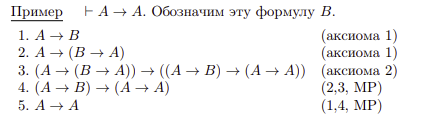
\includegraphics[width=0.6\linewidth]{images/1_definitions_mp}
\end{center}


\subsection{Резолюции.}
\textbf{Определение:} Если $(A \lor x)$ и $(B \lor \neg x)$ одновременно истинны, то $(A \lor B)$ тоже истинно. Такое рассуждение называется правилом резолюции: $\frac{(A \lor x) \quad (B \lor \neg x)}{(A \lor B)}$

\textbf{Определение:} Дизъюнкт $(A \lor B)$ называется резольвентой дизъюнктов $(A \lor x)$ и $(B \lor \neg x)$.

\textbf{Замечание:} Резольвента дизъюнктов $x$ и $\neg x$ -- это пустой дизъюнкт, т.е. $\bot$.

\textbf{Метод резолюций для проверки КНФ на выполнимость:} Будем добавлять к набору дизъюнктов все возможные резольвенты.

\textbf{Теорема:} Метод резолюций всегда заканчивает свою работу, причём для невыполнимых КНФ выводится $\bot$, а для выполнимых не выводится. Таким образом, метод резолюций позволяет проверить выполнимость формулы.

\subsection{Языки первого порядка: индивидные переменные, логические связки, кванторы, функциональные и предикатные символы, термы, атомарные формулы, формулы общего вида.}

Если кванторы $\forall$ и $\exists$ могут стоять только по переменным, то говорят о языке первого порядка. Если же они могут стоять по более сложным объектам, таким как множества или функции, то говорят о языке второго порядка. Возможны и языки высших порядков.

\textbf{Определение:} Языки первого порядка — правила составления формул с кванторами, где кванторы берутся по отдельным объектам.
\newline \par \noindent Алфавит языка первого порядка:
\begin{itemize}
    \item Индивидная переменная (обычно буквы $x, y, z, t, u, v, w$) -- символ формального языка, служащий для обозначения произвольного элемента.
    \item Сигнатура $\sigma = \langle P_1,\ldots, P_k,f_1,\ldots,f_m \rangle$ -- набор предикатных и функциональных символов, обозначающих те или иные связи между объектами. 
    \begin{enumerate}
        \item Предикат валентности $N$ на множестве $A$ -- это функция $P:A^N\to \{0,1\}$ .
        \newline Предикатный символ — символ, обозначающий предикат. 
        \newline Например: $P^{(3)}, <^{(2)}, \subset ^{(2)}, Prime^{(1)}$.
        \newline Предикатные символы нулевой валентности обычно не рассматривают.
        
        \item Функция валентности $N$ на множестве $A$ -- это функция $f:A^N\to A$.
        \newline Функциональный символ — символ алфавита, обозначающий функцию.
        \newline Например: $f^{(3)}, +^{(2)}, \cap ^{(2)}, \sin^{(1)}$.
        \newline Функциональные символы валентности ноль -- это константы: $11, \pi, e, \emptyset$.
    \end{enumerate}
    
    \item Символы логических операций: $\land, \lor, \neg, \to$
    \item Кванторы: $\forall, \exists$
    \item Служебные символы: скобки и запятые.
\end{itemize}

\textbf{Определение:} Терм -- строка, рекурсивно построенная по следующим правилам:
\begin{enumerate}
    \item Индивидная переменная есть терм;
    \item Функциональный символ валентности ноль (т.е. $f^{(0)}=const$) есть терм;
    \item Если $k > 0$, $f^{(k)}$ — функциональный символ валентности $k$, а $t_1,\ldots,t_k$ — термы, то $f^{(k)}(t_1, \ldots,t_k)$ также терм.
\end{enumerate}

\textbf{Определение:} Атомарной формулой называется выражение вида $P^{(k)}(t_1, \ldots,t_k)$ , где $k>0$, $t_1,\ldots,t_k$ — термы, а $P^{(k)}$ —- предикатный символ валентности $k$.

\textbf{Определение:} Формулой (первого порядка) называется строка, рекурсивно построенная по следующим правилам:
\begin{enumerate}
    \item Атомарная формула является формулой;
    \item Если $\phi$ и $\psi$ являются формулами, то строки $(\phi \land \psi), (\phi \lor \psi), (\phi \to \psi), \neg\phi$ также являются формулами;
    \item Если $\phi$ является формулой, а $x$ — индивидная переменная, то $\exists x \ \phi$ и $\forall x \ \phi$ также являются формулами.
\end{enumerate}


\subsection{Интерпретация языка первого порядка. Оценка переменных. Общезначимые формулы.}
\textbf{Определение:} Пусть фиксирована некоторая сигнатура $\sigma$. Чтобы задать интерпретацию сигнатуры $\sigma$, необходимо:
\begin{itemize}
    \item указать некоторое непустое множество $M$, называемое носителем интерпретации;
    \item для каждого $k$-местного предикатного символа $P\in \sigma$ задана некоторая функция $[P]:M^k\to \{0,1\}$;
    \item для каждого $k$-местного функционального символа $f\in \sigma$ задана некоторая функция $[f]:M^k\to M$;
\end{itemize}

\textbf{Определение:} Оценкой переменных называется функция $\pi : Var \to M$, где $Var$ — множество индивидных переменных.
\begin{enumerate}
    \item $[\phi](\pi)$ -- значение формулы $\phi$ на оценке $\pi$
    \item $[t](\pi)$ -- значение терма $t$ на оценке $\pi$
\end{enumerate}

\textbf{Замечание:} Множество $Var$ заранее фиксировано, все термы и формулы строятся на его основе, а оценка
задаёт значения всех переменных из этого множества.
\newline \par Пусть фиксированы интерпретация $I$ и оценка $\pi$. Тогда для каждого терма $t$ должно возникнуть его значение, которое мы будем обозначать через $[t](\pi)$ (зависимость
от интерпретации в явном виде писать не будем, поскольку она не будет меняться в дальнейших определениях, а оценка будет). Поскольку терм строился рекурсивно, его
значение также будет определяться последовательно для всех шагов рекурсии.
\begin{itemize}
    \item[*] Если $t\eqcirc x$, где $x$ -- переменная, то $[t](\pi)=\pi(x)$
    \item[*] Если $t\eqcirc c$, где $c$ -- функциональный символ валентности 0, то $[t](\pi)=[c]$
    \item[*] Если $t\eqcirc f(t_1,\ldots,t_k)$, то $[t](\pi)=[f]([t_1](\pi),\ldots,[t_k](\pi))$
\end{itemize}
Значение формулы также определяется рекурсивно.
\begin{itemize}
    \item[*] Если $\phi\eqcirc P(t_1,\ldots,t_k)$ -- атомарная формула, то $[\phi](\pi)=[P]([t_1](\pi),\ldots,[t_k](\pi))$
    \item[*] Если $\phi\eqcirc \neg\psi$, то $[\phi](\pi)=not([\psi](\pi))$ 
    \item[*] Если $\phi\eqcirc \psi \lor\gamma$, то $[\phi](\pi)=or([\psi](\pi),[\gamma](\pi))$ (аналогично для $\land, \to$)
\end{itemize}

\textbf{Замечание:} Символы логических операций слева от знака равенства являются просто символами, а
справа мы обозначаем соответствующую булеву функцию.
\newline \par  Наконец, перейдём к самому интересному -- кванторам. Это единственный случай,
где изменяется не только формула, значение которой определяется, но и оценка.

\hfill \break
\begin{minipage}{0.6\textwidth}
  \begin{itemize}
    \item[*] Если $\phi\eqcirc \forall x \psi$, то $[\phi](\pi)=\land_{m\in M}[\psi](\pi_{x\to m})$
    \item[*] Если $\phi\eqcirc \exists x \psi$, то $[\phi](\pi)=\lor_{m\in M}[\psi](\pi_{x\to m})$
    \end{itemize}
\end{minipage}
\hfill
\begin{minipage}{0.4\textwidth}
    $\pi_{x\to m} (y)= 
    \begin{cases}
        \pi(y), \; y\neq x \\
        m, \; y=x
    \end{cases}$
\end{minipage}
$$
\land_{m\in M}Q_m=
    \begin{cases}
        1, \; \text{все }Q_m \text{ равны 1} \\
        0, \; \text{иначе}
    \end{cases}
    \qquad 
\lor_{m\in M}Q_m=
    \begin{cases}
        0, \; \text{все }Q_m \text{ равны 0} \\
        1, \; \text{иначе}
    \end{cases}
$$

\hfill \break
\textbf{Определение:} Общезначимая формула -- формула, истинная при любой интерпретации на любой оценке.

\textit{Пример 1:} Для любой формулы $\phi$ формулы $\forall x\forall y\phi \to \forall y\forall x\phi$ и $\exists x\exists y\phi \to \exists y\exists x\phi$ общезначимы.

\textit{Пример 2:} Для любой формулы $\phi$ общезначима формула $\exists x\forall y\phi \to \forall y\exists x\phi$. Обратная импликация общезначима не всегда.

\subsection{Свободные и связные вхождения переменных. Параметры формулы.}
\textbf{Определение:} Говорят, что переменные, от которых не зависят значения формул, связаны некоторым оператором ($\sum, \lim, \max$ или каким-нибудь ещё) и потому называются связанными (имеются в виду переменная $i$ в выражении $\sum_{i=0}^{n} a^{i}$ и тому подобные), а остальные переменные свободны. Более корректно говорить не о связанных и свободных переменных, а о связанных и свободных вхождениях переменных.
\newline 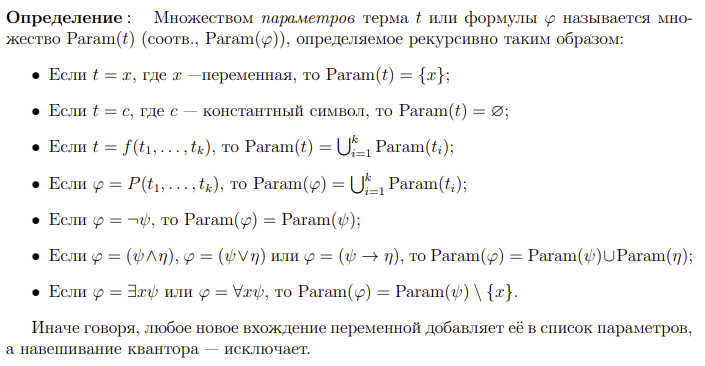
\includegraphics[width=0.9\linewidth]{images/1_definitions_param.png}

\subsection{Выразимость предиката или функции в данной интерпретации.}
Зафиксируем некоторую сигнатуру $\sigma$ и ее интерпретацию с носителем $M$.

\textbf{Определение:} Формула $\phi$ с параметрами $x_1,\ldots,x_m$ выражает предикат $P:M^m\to \{0,1\}$, если $\phi(a_1,\ldots,a_m)=1 \Leftrightarrow P(a_1,\ldots,a_m)=1$.

\textbf{Определение:} Функция $f : M^n \to M$ называется выразимой, если существует формула $\phi$ от $n+1$ переменной, истинная на любой оценке $\pi$, такой что $\pi(x_1) = a_1, \ldots , \pi(x_n) = a_n, \pi(x_{n+1}) = f(a_1,\ldots, a_n)$, и ложная на любой другой оценке.

\textit{Пример 1:} $x\geqslant y \Leftrightarrow \exists z: x=y+z$ в $\mathbb{N}$. Предикат $\geqslant$ выразим в интерпретации $\langle\mathbb{N},+,=\rangle$ и невыразим в интерпретации $\langle\mathbb{Z},+,=\rangle$.

\textit{Пример 2:} Пусть $\langle 2^A,\subset\rangle$: \;\; $x=y \; \Leftrightarrow \; (x\subset y \land y\subset x)$; \;\; $x=\emptyset \; \Leftrightarrow \; \forall y (x\subset y)$.

\subsection{Аксиомы исчисления предикатов, правила Бернайса, правило обобщения.}
Аксиомы исчисления предикатов:
\begin{itemize}
    \item $A_1-A_{11}$ -- аксиомы исчисления высказываний.
    \item $A_{12}: \;\; \forall x \phi \to \phi(t/x)$,  где $t/x$ -- это корректная подстановка терма $t$ в $\phi$ вместо свободных вхождений $x$. 
    \item $A_{13}: \;\; \phi(t/x) \to \exists x \phi$.
\end{itemize}
Корректная подстановка означает, что терм $t$ не содержит переменных, по которым стоят кванторы в $\phi$.

\textit{Пример:} Следствием из $A_{12},A_{13}$ является силлогизма: $\forall x \phi \to \exists x \phi$.

\textbf{Правила вывода:}
\begin{enumerate}
    \item Modus ponens: $$\frac{A\quad A\to B}{B}$$
    \item 1-ое правило Бернайса: $$\frac{\phi\to\psi}{\exists x \; \phi\to\psi}$$
    \item 2-ое правило Бернайса: $$\frac{\phi\to\psi}{ \phi\to\forall x \;\psi}$$
    \item Правило обобщения: $$\frac{\phi}{\forall x \;\phi}$$
\end{enumerate}

\label{exist_x_forall_y}
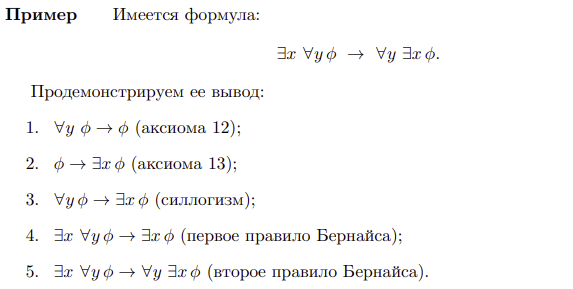
\includegraphics[width=0.65\linewidth]{images/1_definitions_sillog.png}

\subsection{Аксиомы равенства.}
\textbf{Определение:} Пусть $\sigma$ — произвольная сигнатура. Аксиомами равенства в сигнатуре $\sigma$ будут формулы:
\begin{enumerate}
    \item $\forall x \;\; (x=x)$ -- аксиома рефлексивности,
    \item $\forall x \forall y \;\;  \big((x=y)\to(y=x)\big)$ -- аксиома симметричности,
    \item $\forall x \forall y \forall z\;\;  \big(\big((x=y)\land(y=z)\big)\to(x=z)\big)$ -- аксиома транзитивности,
\end{enumerate}

\noindent а также для каждого функционального символа сформулируем аксиому равенства, которая говорит, что его значение не меняется, если аргументы заменить на равные.

\textit{Пример:} Для двухместного функционального символа $f$: $$\forall x_1 \forall x_2 \forall y_1\forall y_2\;\; \big(\big((x_1=x_2)\land(y_1=y_2)\big)\to \big(f(x_1,y_1)=f(x_2,y_2)\big)\big)$$
\noindent Для предикатных символов аксиомы равенства говорят, что истинный предикат остается истинным, если заменить аргументы на равные.

\textbf{Определение:} Формальная арифметика -- это аксиоматическая теория, расширяющая исчисление предикатов с равенством.

\subsection{Теории, модели, нормальные модели.}
Рассмотрим сигнатуру $\sigma$.

\textbf{Определение:} Множество Г замкнутых формул в сигнатуре называется теорией.

\textbf{Определение:} Формула называется замкнутой, если множество ее параметров пусто. Иначе говоря, все переменные замкнутой формулы должны быть связаны кванторами.

\textit{Пример:} $P,\;\; \forall xR(x),\;\; \exists x \forall y P(x,y),\;\; \forall x Q(x)\to \neg(\forall x \exists y R(x,y))$

\textbf{Определение:} Интерпретация $M$ сигнатуры $\sigma$ называется моделью теории Г, если все формулы из Г истинны в $M$.

\textbf{Определение:} Интерпретация $M$ сигнатуры $\sigma$ называется нормальной, если предикат равенства интерпретируется как тождественное совпадение элементов носителя.

\textbf{Определение:} Интерпретация $M$ сигнатуры $\sigma$ называется нормальной моделью теории Г, если она нормальная и все формулы из Г истинны в $M$.

\subsection{Аксиомы арифметики Пеано.}
Стандартная интерпретация: $\mathbb{N}, \; S$ -- следующее число, $0, +, -, =$ понимаются как обычно.

Аксиомы связанные с порядком:
\begin{enumerate}
    \item $\not\exists x \; Sx=0 $
    \item $\forall x \forall y \; (Sx=Sy \to x = y)$
    \item Принцип индукции: $(\phi(0)\land \forall x (\phi(x)\to\phi(Sx)))\to\forall x \phi(x) $
\end{enumerate}

Аксиомы, связанные с арифметическими действиями:
\begin{enumerate}
    \item $\forall x \; x+0=x$
    \item $\forall x \forall y \; x+Sy=S(x+y)$
    \item $\forall x \; x\cdot 0 = 0$
    \item $\forall x \forall y \; x\cdot Sy = x\cdot y + x$
\end{enumerate}

\textit{Пример:} Как вывести, что $2+2 = 4$? В нашем языке это означает, что $SS0+SS0=SSSS0$
\begin{enumerate}
    \item $\forall x \forall y \; x+Sy = S(x+y)$ -- аксиома
    \item $SS0+SS0 = S(SS0+S0)$ -- подстановка $x=SS0, \; y=S0$
    \item $SS0+S0 = S(SS0+0)$ -- подстановка $x=SS0, \; y=0$
    \item $\forall x \; x+0 = x$ -- аксиома
    \item $SS0 + 0 = SS0$ -- подстановка $x=SS0$
    \item $\forall x \forall y \; (x=y \to Sx = Sy)$ -- аксиома равенства
    \item $SS0+0 = SS0\to S(SS0 + 0)=SSS0$ -- подстановка $x=SS0+0,\; y=SS0$
    \item $S(SS0+0)=SSS0$ -- modus ponens
    \item $SS0 + S0 = SSS0$ -- по транзитивности
    \item $S(SS0+S0)=SSSS0$ -- подстановка $x=S(SS0+0), \; y=SSS0$
    \item $SS0 + SS0 = SSSS0$ -- по транзитивности c 2.
\end{enumerate}

\subsection{Совместность, непротиворечивость, полнота теории.}

\textbf{Определение:} Теория Г называется совместной, если все формулы из Г могут быть одновременно истинны в некоторой интерпретации.

\textit{Пример 1:} $\{p \to q,\; q\to p,\; p\land q\}$ -- совместно, так как все верны на $(1,1)$.

\textit{Пример 2:} $\{ \neg (p \to q),\; \neg (q\to p)\}$ -- несовместно, тк первая формула верна только на $(1,0)$, а вторая -- только на $(0,1)$.

\textbf{Утверждение 1:} Г$=\{\phi\}:$ Г совместно $\Leftrightarrow \phi$ выполнима.

\textbf{Утверждение 2:} Г$=\{\phi_1,\ldots,\phi_n\}:$ Г совместно $\Leftrightarrow (\phi_1\land\ldots\land\phi_n)$ выполнима.
\newline \par \textbf{Определение:} Теория Г называется противоречивой, если из нее выводится некоторая формула $\phi$ и ее отрицание $\neg\phi$, и непротиворечивой в противном случае.

\textbf{Определение:} Непротиворечивая теория Г называется полной (в данной сигнатуре), если для любой замкнутой формулы  этой сигнатуры либо Г $\vdash\phi$, либо Г $\vdash\neg\phi$.
    \newpage
    \section{Простые утверждения}

\subsection{Любую булеву функцию можно выразить формулой в КНФ или в ДНФ.}

\begin{center}
    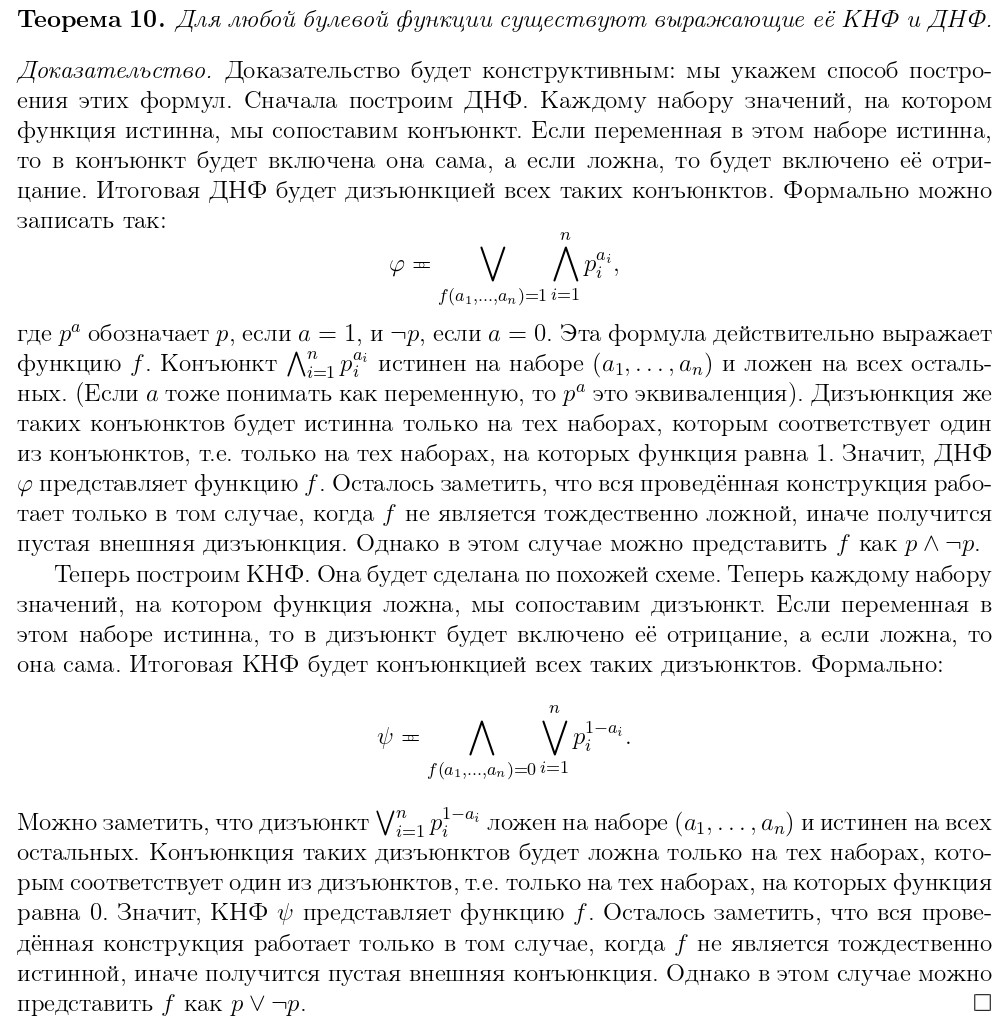
\includegraphics[width=0.95\linewidth]{images/1_propositions_knf}
\end{center}

\subsection{Замкнутость классов Поста относительно композиции.}

\textbf{Определение:} Композиция функций из множества $F$:
\begin{itemize}
    \item Композиция порядка 0 -- все проекторы, т.е. функции вида $pr_i(x_1,\ldots,x_n)=x_i$.
    \item Композиция порядка $m+1$ -- функция вида $h(p_1,\ldots,p_n)=f(g_1(p_1,\ldots,p_n),\ldots,g_k(p_1,\ldots,p_n))$, где $f\in F$, $f$ зависит от $k$ аргументов, $g_1,\ldots,g_k$ -- композиции порядка $\leqslant m$, хотя бы одно из них в точности $m$.
\end{itemize}

\textbf{Определение:} Замыканием класса $Q$ называется класс $[Q]$, составленный из всех композиций любого уровня вложенности функций из класса $Q$.

\textbf{Определение:} Класс булевых функций $Q$ называется замкнутым, если $Q = [Q]$.
\newline \par Докажем замкнутость классов Поста для $f \in T_1, T_0, S, M, L$:
\begin{itemize}
    \item $[T_1] = T_1: \;\; h(1,\ldots,1)=f(g_1(1,\ldots,1),\ldots,g_k(1,\ldots,1))=f(1,\ldots,1)=1$.
    \item $[T_0] = T_0: \;\;$ аналогично $T_1$.
    \item $[M] = M: \;\; 
            \left\{
              \begin{array}{ccc}
                    x_1\leqslant y_1\\
                    \ldots \\
                    x_n\leqslant y_n
              \end{array}
            \right\} \Rightarrow 
            \left\{
              \begin{array}{ccc}
                    g_1(x_1,\ldots,x_n)\leqslant g_1(y_1,\ldots,y_n)\\
                    \ldots \\
                    g_k(x_1,\ldots,x_n)\leqslant g_k(y_1,\ldots,y_n)
              \end{array}
            \right\} \Rightarrow$
            
            $f(g_1(x_1,\ldots,x_n),\ldots,g_k(x_1,\ldots,x_n)) \leqslant f(g_1(y_1,\ldots,y_n),\ldots,g_k(y_1,\ldots,y_n)) $.
    \item $[S] = S: \;\; f(g_1(\neg p_1,\ldots,\neg p_n),\ldots,g_k(\neg p_1,\ldots,\neg p_n)) = f(\neg g_1(p_1,\ldots,p_n),\ldots,\neg g_k(p_1,\ldots,p_n)) = \neg f(g_1(p_1,\ldots,p_n),\ldots,g_k(p_1,\ldots,p_n))$.
    \item $[L] = L$: \;\; Достаточно заметить, что при при подстановке вместо переменных линейной функции каких-то других линейных функций, не могут появиться конъюнкции переменных в слагаемых. Поэтому при такой подстановке получается линейная функция.
\end{itemize}

\subsection{Вывод формулы вида $A \to A$ в исчислении высказываний.}
Доказательство приведено в определении \ref{a_to_a}.

\subsection{Теорема о корректности исчисления высказываний.}
\textbf{Теорема:} Если $\vdash \phi$, то $\phi$ -- тавтология.
\newline $\blacktriangle$ Любая аксиома есть тавтология. Проверяется непосредственно по таблице истинности. Правило MP тоже корректно: если $A$ и $A \to B$ всегда истинны, то $B$ тоже всегда истинно. Индукцией по номеру формулы в выводе доказывается, что все формулы в выводе тавтологичны, что и требовалось. $ \blacksquare$

\subsection{Сведение задачи о выполнимости произвольной формулы к задаче о выполнимости 3-КНФ.}
\textbf{Утверждение:} Пусть $\phi$ -- КНФ. Тогда выполнимость $\phi$ эквивалентна выполнимости $\phi'$, образованной следующим образом: каждый дизъюнкт $(l_1 \lor l_2 \lor \ldots \lor l_k)$ заменяется на такую КНФ: $(l_1 \lor x_1) \land (\neg x_1 \lor l_2 \lor x_2) \land\ldots\land (\neg x_{k-2} \lor l_{k-1} \lor x_{k-1}) \land (\neg x_{k-1} \lor l_k)$, где переменные $x_1, \ldots, x_{k-1}$ свои для каждого дизъюнкта.

$\blacktriangle$ Пусть $\phi$ выполнима. Тогда при выполняющем наборе один из литералов $l_1, \ldots, l_k$ истинен, например, $l_j$. Пусть тогда все $x_i$ с $i < j$ равны $1$, а все $x_i$ с $i \geqslant j$ равны $0$. Это сделает истинным все скобки в новой КНФ.

Пусть, напротив, выполнима $\phi'$. Каждая из переменных $x_i$ может сделать истинной ровно одну скобку. Значит, все они могут сделать истинными максимум $k - 1$ скобку. Оставшаяся должна стать истинной за счёт $l_j$. А значит, и исходный дизъюнкт выполнен. $\quad \blacksquare$


\subsection{Представление задачи о раскраске графа и задачи о расстановке ферзей на шахматной доске как задачи о выполнимости КНФ.}
\begin{itemize}
    \item \textit{Задача о 3-раскраске вершин графа.} Пусть задан некоторый неориентированный граф. Ставится вопрос: можно ли его вершины раскрасить в 3 цвета, так чтобы
    вершины одного цвета не были соединены ребром. КНФ строится так: для каждой вершины $i$ заводится две переменных $p_i$ и $q_i$. Будем считать, что пара значений
    $(0, 1)$ кодирует первый цвет, пара $(1, 0)$ второй цвет, а пара $(1, 1)$ третий цвет. Чтобы исключить вариант $(0, 0)$, добавим условия $(p_i \lor q_i)$. Далее, для каждого
    ребра $(i, j)$ пара $(p_i, q_i)$ должна отличаться от пары $(p_j, q_j)$. Это выражается такой КНФ: $$(p_i\lor p_j \lor q_i \lor q_j )\land(p_i\lor p_j \lor \neg q_i \lor \neg q_j )\land (\neg p_i\lor \neg p_j\lor q_i\lor q_j )\land(\neg p_i\lor \neg p_j \lor \neg q_i \lor\neg q_j )$$
    Выполнимость конъюнкции всех таких формул эквивалентна раскрашиваемости исходного графа.
    
    \item \textit{Задача о расстановке ферзей на шахматной доске.} Известна такая задача: можно ли расставить $8$ ферзей на шахматной доске, так чтобы они не били друг друга. Мы заведём переменные $p_{ij}$, истинность которых означает, что в клетке с координатами $(i, j)$ стоит ферзь. 
    \newline -- По условию в одной строке не может быть двух ферзей, значит, в каждой должен быть ровно один. Достаточно написать дизъюнкты вида $(p_{i1} \lor p_{i2} \lor \ldots\lor p_{i8})$. \newline -- Далее, запишем условия, что в каждом столбце стоит не более одного ферзя. А именно, для каждого набора $(i, j \neq i, k)$ возьмём дизъюнкт $(\neg p_{ik} \lor \neg p_{jk})$. Аналогичные условия для строк можно записать отдельно, но они будут следовать из уже написанных. \newline -- Также нужно написать условия для диагоналей: $(\neg p_{ij} \lor \neg p_{i+k,j+k})$ и $(\neg p_{ij} \lor\neg p_{i+k,j-k})$ при всех $i$, всех $j < 8$ и всех $k> 0$ (записываются только те условия, где все индексы попадают в интервал от 1 до 8). \newline Любой выполняющий набор для такой системы задаёт расстановку ферзей. Можно рассматривать разные варианты задачи: другой размер доски, фиксированное положение некоторых ферзей (тогда добавятся дизъюнкты $p_{ij}$) или запрещённые клетки (тогда добавятся дизъюнкты $\neq p_{ij}$).
\end{itemize}

\subsection{Теорема о корректности метода резолюций: из выполнимой КНФ нельзя вывести $\bot$.}
\textbf{Теорема:} Метод резолюций всегда заканчивает свою работу, причём для невыполнимых КНФ выводится $\bot$ (полнота), а для выполнимых не выводится (корректность). Таким образом, метод резолюций позволяет проверить выполнимость формулы: достаточно добавить все возможные резольвенты и проверить, встретился ли $\bot$.

$\blacktriangle$ Всего существует конечное число дизъюнктов, так что в какой-то момент новые перестанут появляться, поэтому метод всегда заканчивает свою работу. Как обычно, корректность доказывается легко. Действительно, если исходная КНФ была выполнима, то она останется выполнимой после добавления любого числа резольвент. Но КНФ с $\bot$ выполнимой быть не может. Значит, для выполнимой КНФ $\bot$ не появится. $\quad \blacksquare$


\textit{Пример:} Невыполнимая КНФ $(x_1 \lor x_2 \lor x_3) \land (\neg x_1 \lor x_2) \land (\neg x_2 \lor x_3) \land \neg x_3$ опровергается так:
\begin{enumerate}
    \item $(x_1 \lor x_2 \lor x_3) \land (\neg x_1 \lor x_2) \vdash (x_2 \lor x_3)$
    \item $(x_2 \lor x_3) \land (\neg x_2 \lor x_3) \vdash x_3$
    \item $x_3 \land \neg x_3 \vdash \bot$
\end{enumerate}

\subsection{Значение терма (формулы) первого порядка зависит только от значений его (её) параметров.}

\textbf{Теорема:} Истинность формулы (значение терма) зависит только от её (его) параметров. Иными словами, если оценки $\pi$ и $\rho$ таковы, что $\forall x \in $ Param$(\phi) \;
(\text{или }x \in $ Param$(t))$ выполнено $\pi(x) = \rho(x)$, то $[\phi](\pi) = [\phi](\rho) \; (\text{или }[t](\pi) = [t](\rho))$.
\newline $\blacktriangle$ Будем доказывать утверждение индукцией по построению терма, а затем формулы:
\begin{itemize}
    \item Если $t = x$, то $[t](\pi) = \pi(x) = \rho(x) = [t](\rho)$.
    \item Если $t = c$, то $[t](\pi) = [c] = [t](\rho)$.
    \item Если $t = f(t_1,\ldots, t_k)$, то в силу Param$(t_i) \subset$ Param$(t)$ по предположению индукции имеем $[t_i](\pi) = [t_i](\rho)$. Поэтому $[t](\pi) = [f]([t_1](\pi),\ldots, [t_k](\pi)) = [f]([t_1](\rho),\ldots, [t_k](\rho)) = [t](\rho)$;
    \item Если $\phi = P(t_1,\ldots, t_k)$, то рассуждение аналогично предыдущему;
    \item Если $\phi = \neg\psi$, то $[\phi](\pi) = \neg[\psi](\pi) = \neg[\psi](\rho) = [\phi](\rho)$. Здесь предположение индукции использовано во втором равенстве;
    \item Если $\phi = (\psi \land\gamma)$, то $[\phi](\pi) = [\psi](\pi) \land [\gamma](\pi) = [\psi](\rho) \land [\gamma](\rho) = [\phi](\rho)$. Здесь во втором равенстве использовано предположение индукции и вложения Param$(\psi) \subset$ Param$(\phi)$ и Param$(\gamma) \subset$ Param$(\phi)$. Случай $\phi = (\psi \lor\gamma)$ и $\phi = (\psi \to\gamma)$ разбираются аналогично;
    \item Если $\phi = \exists x\psi$, то ключевое соображение состоит в следующем: если $\pi(y) = \rho(y)$ для всех $y \in$ Param$(\psi) \setminus \{x\}$, то $\pi_{x\to m}(y) = \rho_{x\to m}(y)$ уже для всех $y \in$ Param$(\psi)$, в том числе для $y = x$. Действительно, $\pi_{x\to m}(y) = \rho_{x\to m}(y) = m$, а для $y\neq x$ равенство есть по предположению. Поэтому $[\phi](\pi) = \bigvee_{m\in M}[\psi](\pi_{x\to m}) = \bigvee_{m\in M}[\psi](\rho_{x\to m})=[\phi](\rho)$. Аналогичное рассуждение работает и для $\phi = \forall x\psi$. $\quad \blacksquare$
\end{itemize}

\subsection{Выразимость свойств «равняться нулю», «равняться единице», «делиться нацело», «быть простым числом», «равняться наибольшему общему делителю», «равняться наименьшему общему кратному» в интерпретации $\langle\mathbb{N},\cdot\;,=\rangle$.}

Рассмотрим интерпретацию $\langle\mathbb{N},\cdot\;,=\rangle$. Будем выражать в ней различные предикаты:
\begin{itemize}
    \item $x = 0 \; \Leftrightarrow \; \forall y \; x \cdot y = x$
    \item $x = 1 \; \Leftrightarrow \; \forall y \; x \cdot y = y$
    \item $x \svdots y \; \Leftrightarrow \; \exists z \; x= y \cdot z$
    \item $Prime(p) \; \Leftrightarrow \; (p\neq 1 \;\land\; \forall q(p\svdots q \to (q=1 \;\lor\; q=p)))$
    \item $d=$ НОД$(x,y) \; \Leftrightarrow \; (x\svdots d \;\land\; y \svdots d \;\land\; \forall k ((x\svdots k \;\land\; y \svdots k)\to d \svdots k))$
    \item $d=$ НОK$(x,y) \; \Leftrightarrow \; (d\svdots x \;\land\; d \svdots y \;\land\; \forall k ((k\svdots x \;\land\; k \svdots y)\to k \svdots d))$
    
\end{itemize}

\subsection{Любую формулу первого порядка можно привести к предваренной нормальной форме.}

\textbf{Определение:} Формула находится в предварённой нормальной форме, если вначале идут кванторы по некоторым переменным в некотором порядке, а затем — бескванторная формула.

\textbf{Теорема:} Для любой формулы существует эквивалентная ей формула в предваренной нормальной форме.

$\blacktriangle$ Алгоритм будет таким: сначала переименовать связанные переменные, так чтобы под всеми кванторами были разные переменные, притом не совпадающие с именами свободных переменных. Затем вынести все кванторы наружу, меняя их при выносе из отрицания или посылки импликации по правилам 4-7 из списка ниже. $\quad \blacksquare$
\newline
\newline
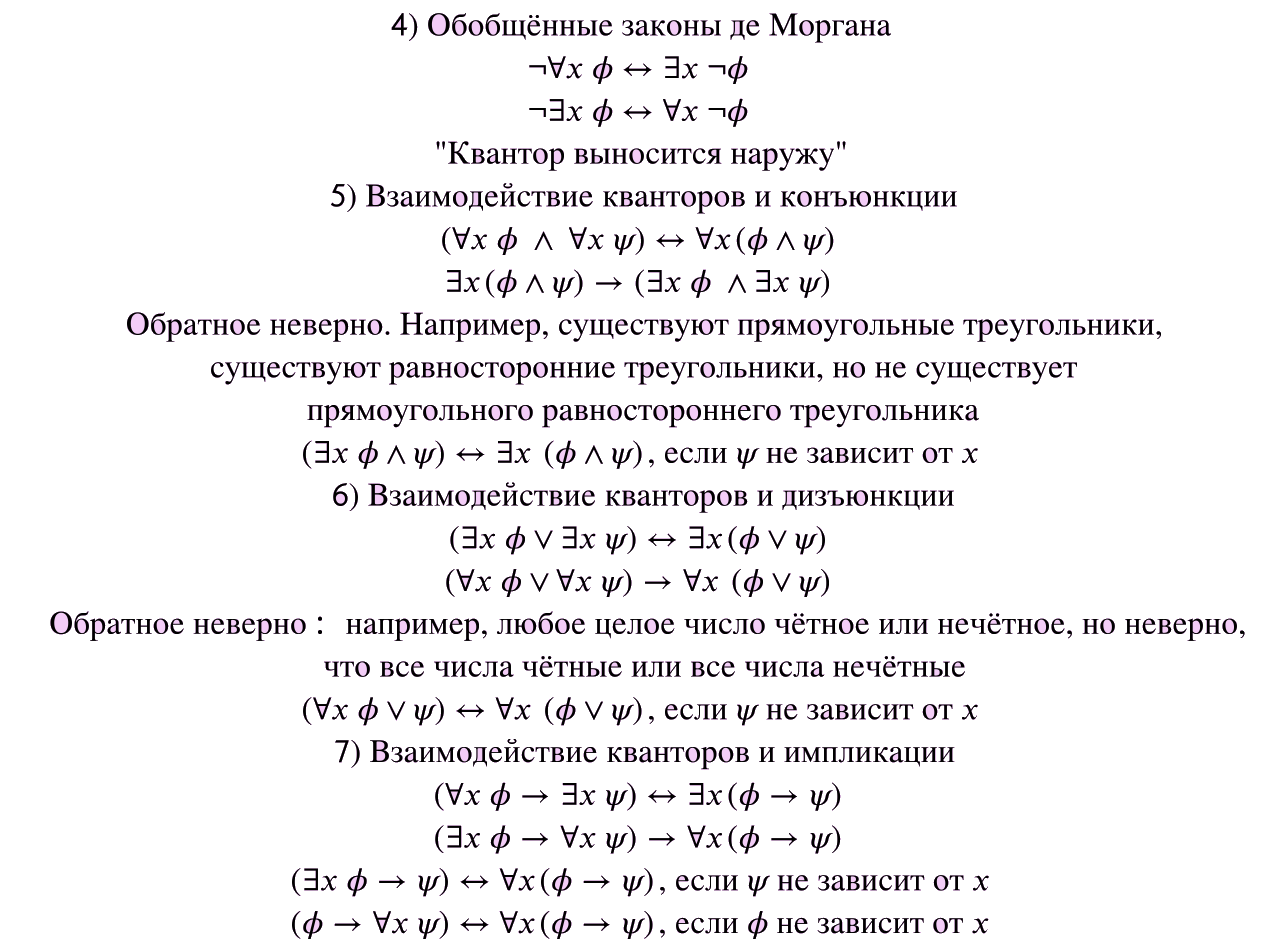
\includegraphics[width=0.9\linewidth]{images/1_propositions_rules}

\textit{Пример:} $\exists x A(x) \land \exists xB(x) \; \Leftrightarrow \; \exists x A(x) \land \exists yB(y) \; \Leftrightarrow \; \exists x (A(x) \land \exists yB(y)) \; \Leftrightarrow \; \exists x\exists y( A(x) \land B(y))$.

\subsection{Вывод правила обобщения в исчислении предикатов.}
Правило обобщения: $$\frac{\phi}{\forall x \;\phi}.$$

$\blacktriangle$ Докажем правило обобщения:
\begin{enumerate}
    \item $\phi$ (считаем, что уже вывели)
    \item $\psi$ (некоторая аксиома, не зависящая от $x$)
    \item $\phi\to(\psi\to\phi)$ (Ax. 1)
    \item $\psi\to\phi$ (MP 1-3)
    \item $\psi\to\forall x \phi$ (2-ое правило Бернайса)
    \item $\forall x \phi$ (MP 2-5) $\quad \blacksquare$
\end{enumerate}

\subsection{Вывод формулы вида $\exists x \forall y \phi \to \forall y \exists x \phi$ в исчислении предикатов.}

Доказательство приведено в определении \ref{exist_x_forall_y}.

\subsection{Любое совместное множество формул первого порядка непротиворечиво.}
$\blacktriangle$ От противного: пусть Г -- противоречиво. Если Г $\vdash \phi$ и все формулы из Г верны на некотором наборе (def: совместности), то $\phi$ верно на том же наборе. При этом Г $\vdash \phi$ и Г $\vdash \neg\phi$, то Г $\phi$ и $\neg\phi$ одновременно верны на этом наборе, противоречие $\Leftrightarrow$ Г -- непротиворечиво. $\quad \blacksquare$

\subsection{Из теоремы Гёделя о полноте исчисления предикатов в сильной форме (любая непротиворечивая теория имеет модель) следует теорема в слабой форме (любая общезначимая формула выводима в исчислении предикатов).}

\textbf{Определение:} Множество Г замкнутых формул в сигнатуре называется теорией.

\textbf{Определение:} Формула называется замкнутой, если множество ее параметров пусто. Иначе говоря, все переменные замкнутой формулы должны быть связаны кванторами.

\textbf{Определение:} Интерпретация $M$ сигнатуры $\sigma$ называется моделью теории Г, если все формулы из Г истинны в $M$.

\textbf{Утверждение:} Из теоремы в сильной форме следует теорема в слабой форме.

$\blacktriangle$ Пусть $\phi$ -- общезначимая формула. Значит, $\forall x\phi$ тоже общезначимая формула (по корректности правила обощения). Значит, $\{\neg \forall x\phi\}$ -- теория, не имеющая модели. По контрапозиции к сильной формулировке получаем, что $\{\neg \forall x\phi\}$ -- противоречива. Таким образом, $\{\neg \forall x\phi\}\vdash \psi,\neg\psi$. Тогда, по лемме о дедукции, можно вывести $\neg\neg \forall x\phi \; \Rightarrow \;\vdash\forall x \phi \; \Rightarrow \; \vdash \phi$ (по аксиоме 12). $\quad \blacksquare$

\subsection{Выразимость в арифметике свойств «быть степенью двойки», «быть степенью четвёрки».}
Пусть задано $\langle\mathbb{N}, 0, S, +, \; \cdot, =\rangle$. Заметим, что $x \svdots y \; \Leftrightarrow \; \exists z \; x= y \cdot z$. Тогда $x$ является степенью 2 $\; \Leftrightarrow \; \forall d(x \svdots d \to (d=1 \;\lor\; d \svdots 2))$.

Аналогично, $x$ является степенью 4 $\; \Leftrightarrow \; \exists y \ \forall d((y\cdot y = x) \land (y \svdots d \to (d=1 \;\lor\; d \svdots 2)))$.

\subsection{Множество предложений, выводимых в арифметике Пеано, перечислимо.}
\textbf{Определение:} Множество называется перечислимым, если существует алгоритм, который печатает все элементы этого множества и только их.

$\blacktriangle$ Пусть $\mathcal{A}$ -- система аксиом в арифметике Пеано. Мы можем алгоритмически перечислять конечные последовательности формул (например, в порядке возрастания суммы длин формул в такой последовательности). Для каждой последовательности формул можно проверить, является ли она выводом из $\mathcal{A}$. Если очередная последовательность формул оказывается выводом из $\mathcal{A}$, то мы добавляем последнюю формулу из этой последовательности к списку выводимых формул. Так мы рано или поздно перечислим каждую формулу, выводимую из данной системы аксиом, что и требовалось. $\quad \blacksquare$

    \newpage
    \section{Вопросы из билетов}

\subsection{Теорема об однозначном представлении булевой функции многочленом Жегалкина.}
\textbf{Теорема (Жегалкина):} Каждая булева функция единственным образом представляется в виде полинома Жегалкина.

$\blacktriangle$ Заметим, что различных булевых функций от $n$ переменных $2^{2^n}$ штук. При этом конъюнкций вида $x_{i_1}\ldots x_{i_k}$ существует ровно $2^n$, так как из $n$ возможных сомножителей каждый или входит в конъюнкцию, или нет. В полиноме у каждой такой конъюнкции стоит 0 или 1, то есть существует $2^{2^n}$ различных полиномов Жегалкина от $n$ переменных.

Теперь достаточно лишь доказать, что различные полиномы реализуют различные функции. Предположим противное. Тогда приравняв два различных полинома и перенеся один из них в другую часть равенства, получим полином, тождественно равный нулю и имеющий ненулевые коэффициенты. Тогда рассмотрим слагаемое с единичным коэффициентом наименьшей длины, то есть с наименьшим числом переменных, входящих в него (любой один, если таких несколько). Подставив единицы на места этих переменных и нули на места остальных, получим, что на этом наборе только одно это слагаемое принимает единичное значение, то есть нулевая функция на одном из наборов принимает значение 1. Противоречие. Значит, каждая булева функция реализуется полиномом Жегалкина единственным образом. $\quad \blacksquare$ 

\subsection{Теорема о дедукции для исчисления высказываний.}

\textbf{Теорема о дедукции:} Пусть $\Gamma$, $A$ -- это $\Gamma \,\cup\, \{A\}$, тогда верно:
$$\frac{\Gamma\vdash A\to B}{\Gamma,A\vdash B}\;\;\Updownarrow$$

$\blacktriangle$ $(\,\Downarrow)$ Пусть $\Gamma \vdash A\to B$, тогда $\Gamma, A \vdash A,\; A\to B$. К выводу применим MP: $A,\;A\to B \vdash B$. Тогда по транзитивности $\Gamma, A\vdash B$. \newline $(\,\Uparrow)$ Доказывается индукцией по длине вывода $B$ из $\Gamma, A$
\begin{itemize}
    \item[(1)] Если этот вывод -- длины $1$, то $B$ -- аксиома или гипотеза (т.е. формула из $\Gamma$). \newline Если B -- аксиома, то имеем вывод $A \to B$ (из $\emptyset$): \newline 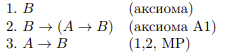
\includegraphics[width=0.35\linewidth]{images/1.1_case1.png}
    \item[(2)] Если $B \in \Gamma$, то имеем такой же вывод $A \to B$ из $\Gamma$: \newline 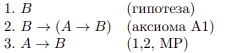
\includegraphics[width=0.35\linewidth]{images/1.1_case2.png}
    \item[(3)] Если $B = A$, то $A \to B = A \to A$. Но $\vdash A \to A$ (пример из определений \ref{a_to_a}).
    \item[(4)] Предположим теперь, что $\Gamma, A \vdash B$ и утверждение $(\,\Uparrow)$ верно для всех более коротких выводов, т.е. для всех $C$, если $\Gamma, A \vdash C$ и вывод $C$ из $\Gamma$, $A$ короче, чем вывод $B$, то $\Gamma$ $\vdash A \to C$.
    \newline Покажем, что $\Gamma \vdash A \to B$. Рассмотрим вывод из $\Gamma, A$, который заканчивается формулой $B$. При этом $B$ может оказаться аксиомой или гипотезой (тогда все предыдущие формулы для доказательства $B$ не нужны). Но в этом случае  $\Gamma \vdash A \to B$ по (1)–(3).
    \newline Остается случай, когда $B$ получается по MP из формул $C, C \to B$, причем $\Gamma, A \vdash C$ и $\Gamma, A \vdash C \to B$ с более короткими доказательствами. По предположению индукции имеем:
    \\
    \\
    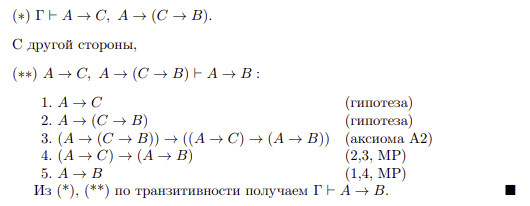
\includegraphics[width=0.8\linewidth]{images/1.1_case3.png}
\end{itemize}

\subsection{Теорема о полноте исчисления высказываний.}

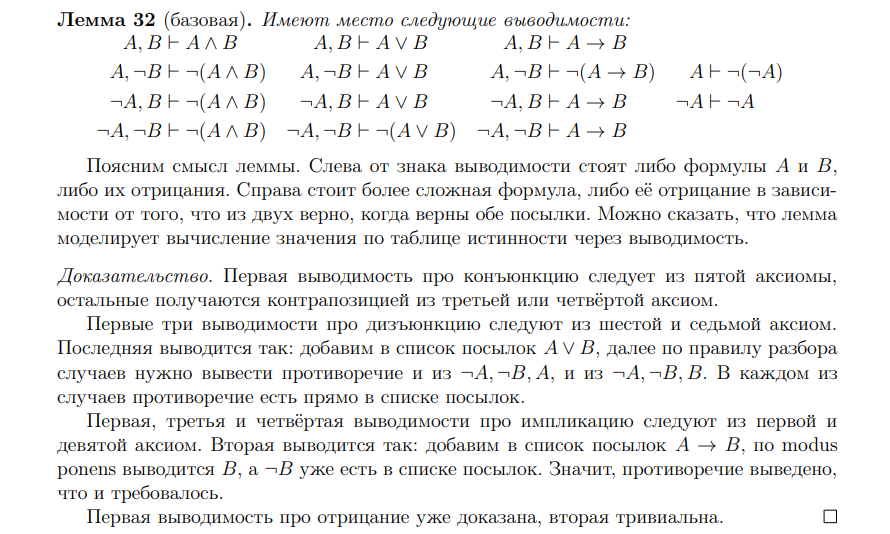
\includegraphics[width=0.93\linewidth]{images/lem_1_base.png}

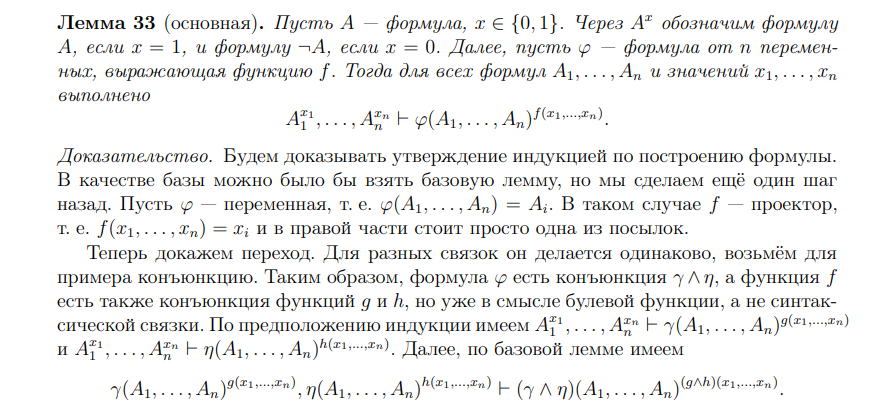
\includegraphics[width=0.93\linewidth]{images/lem_2_main_1.png}

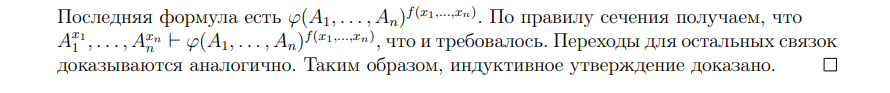
\includegraphics[width=0.93\linewidth]{images/lem_2_main_2.png}


\includegraphics[width=0.93\linewidth]{images/def_for_proof_1.png}


\includegraphics[width=0.93\linewidth]{images/th_main_for_full.png}


\includegraphics[width=0.93\linewidth]{images/proof_for_prop_1.png}

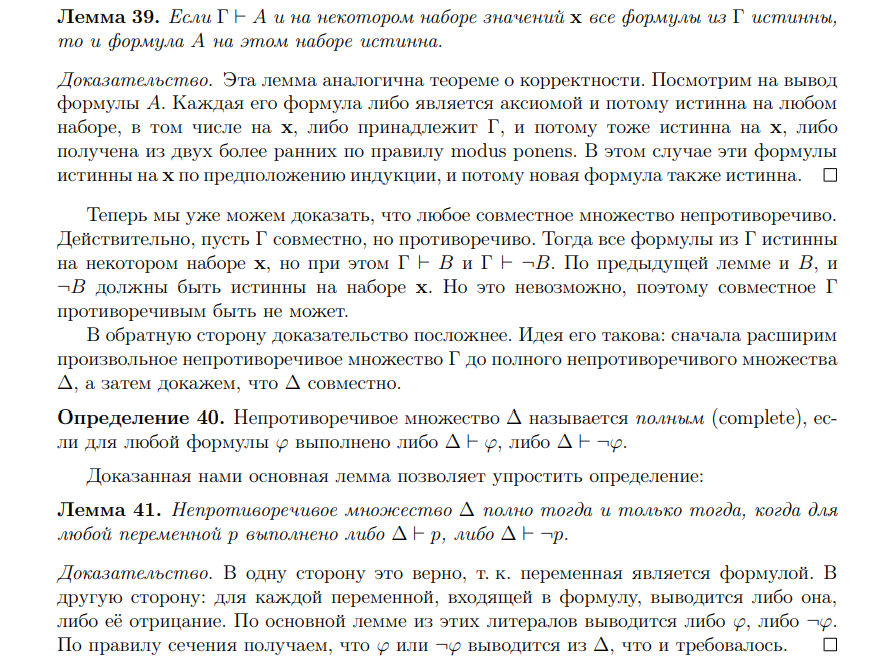
\includegraphics[width=0.93\linewidth]{images/three_lemms_for_full.png}

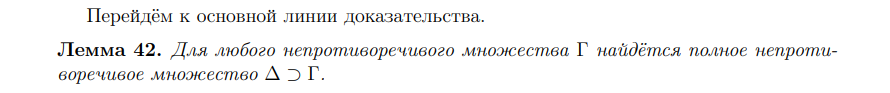
\includegraphics[width=0.93\linewidth]{images/the_last_lemm_full.png}

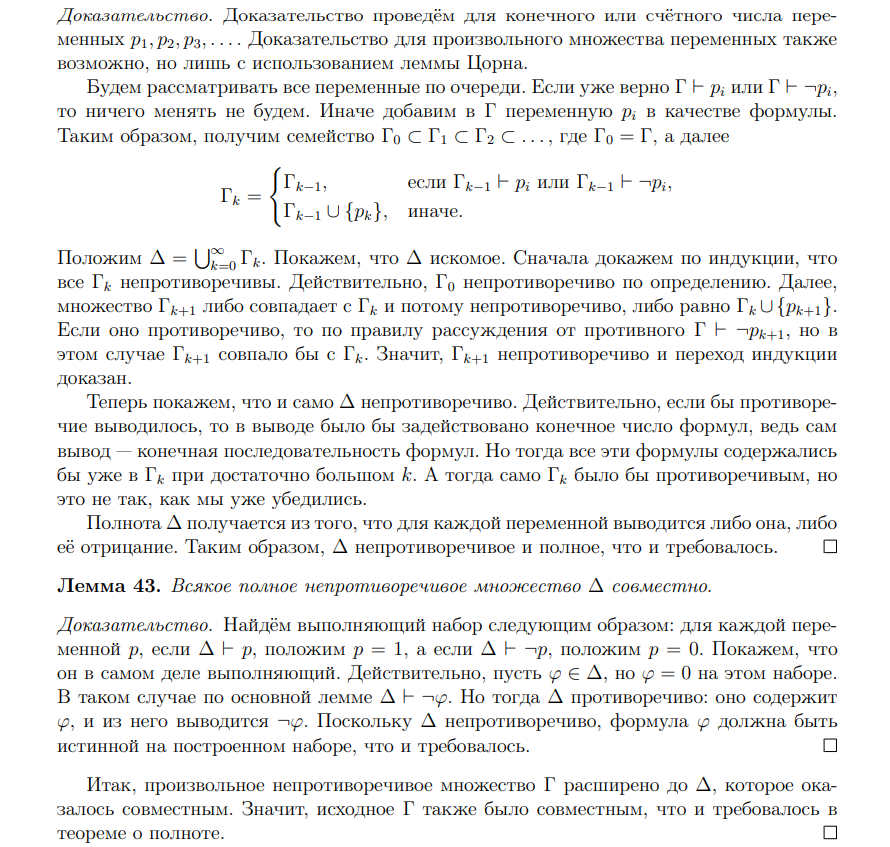
\includegraphics[width=0.93\linewidth]{images/end_of_proof_full.png}


%Из следующей теоремы нам понадобятся только 4) и 6) правила.
%\par

%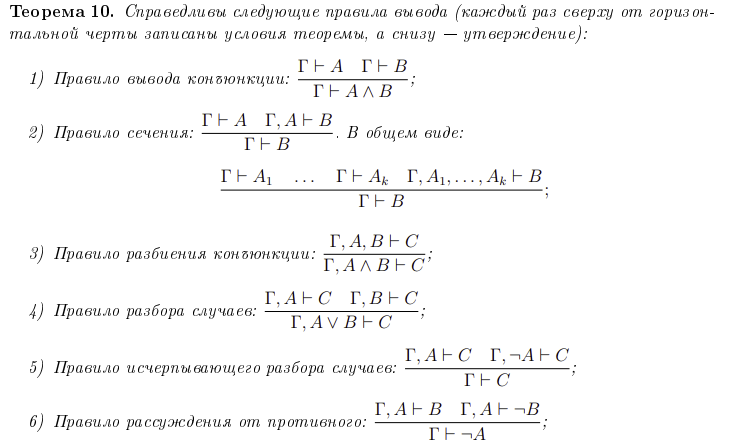
\includegraphics[width=1\linewidth]{images/1.2_theorem}

%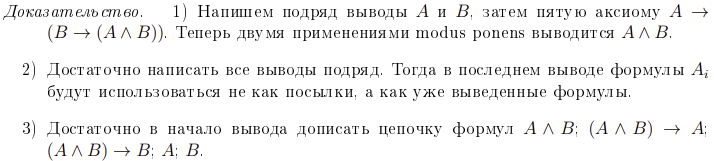
\includegraphics[width=0.97\linewidth]{images/1.1_v1}

%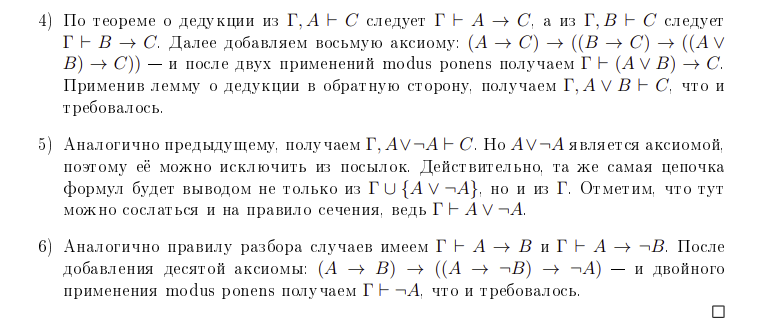
\includegraphics[width=0.97\linewidth]{images/1.1_v3}

%
\includegraphics[width=0.97\linewidth]{images/1.1_neg}

%\par \noindent Для доказательства теоремы о полноте понадобятся две вспомогательные леммы.

%\textbf{Базовая лемма:} Представление таблицы истинности для данных четырех связок.

%\begin{tabular}{|p{1.5in}|p{1.5in}|p{1.5in}|p{1.5in}|}
%\hline
%    Для дизъюнкции: & Для конъюнкции: & Для импликации: & Для отрицания:\\ 
%    \hline
%    \centering{$A,B \vdash A\lor B$} & \centering{$A,B \vdash A \land B$} & %\centering{$A,B \vdash A\to B$} & \centering{$A \vdash \neg (\neg A)$} \tabularnewline
%    
%    \centering{$\neg A,B \vdash A\lor B$} & \centering{$\neg A,B \vdash \neg (A\land B)$} & \centering{$\neg A,B \vdash A\to B$}& \centering{$\neg A \vdash \neg A$} \tabularnewline
    
%    \centering{$A,\neg B \vdash A\lor B$} & \centering{$A, \neg B \vdash \neg (A\land B)$} & \centering{$A,\neg B \vdash \neg (A\to B)$}& \centering{} \tabularnewline
    
%    \centering{$\neg A,\neg B \vdash \neg (A\lor B)$} & \centering{$\neg A, \neg B \vdash \neg (A\land B)$} & \centering{$\neg A,\neg B \vdash A\to B$}& \centering{} \tabularnewline
%    \hline
%\end{tabular}

%\begin{enumerate}
%    \item Первые три выводимости про дизъюнкцию следуют из $A_6$ и $A_7$ по лемме о дедукции ($D$). Последняя: \newline
%    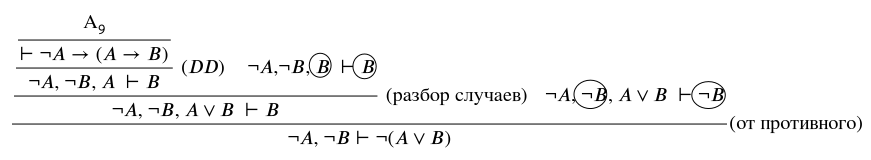
\includegraphics[width=0.99\linewidth]{images/1.1_dedu.png}
%    \item Первая выводимость про конъюнкцию следует из $A_5$ по $D$, остальные получаются контрапозицией из $A_3$ и $A_4$: \newline
%    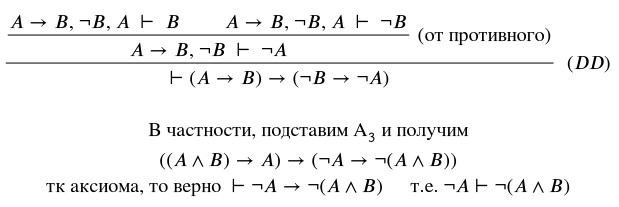
\includegraphics[width=0.8\linewidth]{images/1.1_cntrl.png}
%    \item Первая, третья и четвертая выводимость про импликацию следуют из $A_1$ и $A_9$ по $D$. Вторая выводится так: \newline
%    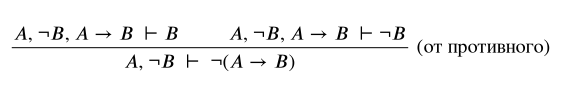
\includegraphics[width=0.7\linewidth]{images/1.1_negg.png}
%    \item Первая выводимость про отрицание доказана в утверждении 14, вторая тривиальна.
%\end{enumerate}

%\par \textbf{Основная лемма:} Пусть $\phi$ - это формула, зависящая от $p_1,\ldots,p_n$. Тогда верно следующее:
%$$p_1^{a_1},p_2^{a_2},\ldots,p_n^{a_n} \vdash \phi^{\phi(a_1,\ldots,a_n)} \text{, \qquad %где } p^a = \begin{cases}
%p, a = 1\\
%\neg p, a = 0
%\end{cases}$$
%Обозначим $a = \phi(a_1,\ldots,a_n)$

%$\blacktriangle$ Доказательство будет вестись индукцией по построению формулы с использованием базовой леммы в качестве базы и в переходе.
%\newline \textit{База индекции:} $\phi$ содержит  одну связку. Тогда это утверждение сводится к базовой лемме.
%\newline \textit{Переход:} пусть $\phi = \psi \land \gamma$. Тогда можно записать: $\phi(a_1,\ldots,a_n) = \psi(a_1,\ldots,a_n) \land \gamma(a_1,\ldots,a_n)$
%\newline Пусть $\psi(a_1,\ldots,a_n) = \alpha, \;\; \gamma(a_1,\ldots,a_n) = \beta$
%\newline Применим предположение индукции: $p_1^{a_1},\ldots,p_n^{a_n} \vdash \psi^\alpha, \;\;\; p_1^{a_1},\ldots,p_n^{a_n} \vdash \gamma^\beta$
%\newline Воспользуемся базовой леммой:
%$\psi^\alpha, \; \gamma^\beta \vdash (\psi \land \gamma)^{(\alpha\land\beta)}=\phi^a $
%\newline Записав все выводы подряд, получаем: $p_1^{a_1},p_2^{a_2},\ldots,p_n^{a_n} \vdash \phi^{a}$
%\newline Аналогичные действия проделаем и для других связок. Имеются база и переход, значит, по индукции докажем лемму для всех формул. $\qquad \blacksquare$

%\textit{Пример:} $\phi=\neg p \land (q\lor r); \quad \phi(0,1,0)=1;\quad \phi(1,0,0)=1$

%Лемма утверждает следующее: $\quad \neg p, q, \neg r \vdash \phi; \qquad p, \neg q, \neg r \vdash \neg \phi$
%\newline \par \textbf{Теорема о полноте ИВ:} Если формула $\phi$ является тавтологией, то тогда $\phi$ -- выводима. 

%$\blacktriangle$ Пусть $\phi$ -- тавтология. Тогда $\forall a_1\ldots a_n \;\; \phi(a_1,\ldots,a_n) = 1$. Значит, по основной лемме $ p_1^{a_1},p_2^{a_2},\ldots,p_n^{a_n} \vdash \phi$ при $\forall a_1\ldots a_n$. Далее воспользуемся правилом исчерпывающего разбора случаев, а также закон исключенного третьего: \newline
%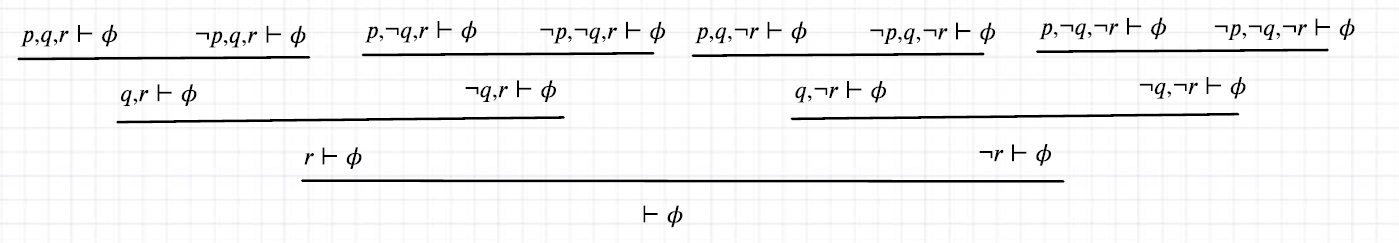
\includegraphics[width=1\linewidth]{images/1.1_cases.png}
%Такое рассуждение можно провести не только для трех литералов, но и для любого количества. Значит, теорема о полноте доказана. $\qquad \blacksquare$



\subsection{Теорема о полноте метода резолюций: из невыполнимой КНФ всегда можно вывести $\perp$.}

\textbf{Теорема.} Метод резолюций всегда заканчивает свою работу, причём для невыполнимых КНФ выводится $\perp$ (полнота), а для выполнимых не выводится (корректность).


\includegraphics[width=0.95\textwidth]{images/resolut_proof_1.png}


\includegraphics[width=0.95\textwidth]{images/resolut_proof_2.png}


\subsection{Теорема о компактности для исчисления высказываний.}

\textbf{Теорема:} Пусть любое конечное подмножество множества $\Gamma$ совместно. Тогда и всё множество $\Gamma$ совместно.

$\blacktriangle$ Если всё множество $\Gamma$ несовместно, то оно противоречиво. Но тогда в нём есть конечное противоречивое подмножество. Но тогда оно несовместно, что противоречит условию. $\quad \blacksquare$

\subsection{Устойчивость выразимых предикатов при автоморфизмах интерпретаций.}

Пусть имеется некоторая сигнатура $\sigma$ и интерпретация этой сигнатуры, носителем которой является множество $M$.

\textbf{Определение:} Взаимно однозначное отображение $\alpha: M \to M$ называется \textit{автоморфизмом} интерпретации, если все функции и предикаты, входящие в интерпретацию, устойчивы относительно $\alpha$. При этом k-местный предикат $P$ называется \textit{устойчивым} относительно $\alpha$, если 
\[P(\alpha(m_1), \ldots, \alpha(m_k)) \lra P(m_{1}, \ldots, m_{k})\]
для любых элементов $m_1, \ldots, m_k \in M$. Далее, k-местная функция $f$ называется устойчивой относительно $\alpha$, если
\[f(\alpha(m_{1}), \ldots, \alpha(m_{k})) = \alpha(f(m_{1}, \ldots, m_{k})).\]

\textbf{Теорема:} Любой предикат, выразимый в данной интерпретации, устойчив относительно её автоморфизмов.

$\blacktriangle$ Пусть $\pi$ — некоторая оценка, то есть отображение, ставящее в соответствие всем индивидным переменным некоторые элементы носителя. Через $\alpha \circ \pi$ обозначим оценку, которая получится, если к значению каждой переменной применить отображение $\alpha$; другими словами, $\alpha \circ \pi (\xi) = \alpha(\pi(\xi))$ для любой переменной $\xi$.

Первый шаг состоит в том, чтобы индукцией по построению терма t доказать такое утверждение: значение терма t при оценке $\alpha \circ \pi$ получается применением $\alpha$ к значению терма t при оценке $\pi$: $[t](\alpha \circ \pi) = \alpha([t](\pi))$.

Для переменных это очевидно, а шаг индукции использует устойчивость всех функций интерпретации относительно $\alpha$. Теперь индукцией по построению формулы $\varphi$ легко доказать такое утверждение: $[\varphi](\alpha \circ \pi) = [\varphi](\pi)$.

Мы не будем выписывать эту проверку; скажем лишь, что взаимная однозначность $\alpha$ используется, когда мы разбираем случай кванторов. (В самом деле, если с одной стороны изоморфизма берётся какой-то объект, то взаимная однозначность позволяет взять соответствующий ему объект с другой стороны изоморфизма.)
$\blacksquare$

\subsection{Теорема Гёделя о полноте исчисления предикатов: расширение любого непротиворечивого множества до полного и экзистенциально полного.}

\textbf{Определение:} Множество Г замкнутых формул в сигнатуре называется теорией.

\textbf{Определение:} Интерпретация $M$ сигнатуры $\sigma$ называется моделью теории Г, если все формулы из Г истинны в $M$.

\textbf{Определение:} Теория Г называется совместной, если все формулы из Г могут быть одновременно истинны в некоторой интерпретации.

\textbf{Определение:} Теория Г называется противоречивой, если из нее выводится некоторая формула $\phi$ и ее отрицание $\neg\phi$, и непротиворечивой в противном случае.

\par
\textbf{Теорема Гёделя о полноте исчисления предикатов}:
Если $\varphi$ общезначима, то она выводима в исчислении предикатов.
Пользуясь данной терминологией, можно сформулировать теорему, из которой будет следовать теорема Гёделя.

\textbf{Теорема}: Если теория непротиворечива, то она совместна (имеет модель).

\textbf{Доказательство:} 1. Мы хотим расширить не противоречивую Г так, чтобы она была полной (если $\varphi$ - замкнутая формула, то Г $ \vdash \varphi$ или  Г $ \vdash \neg \varphi$) и экзистенциально полной (т.е. если Г $ \vdash \exists x \varphi$, то Г $ \vdash \varphi(t/x)$, где t - замкнутый терм.
\begin{center}
    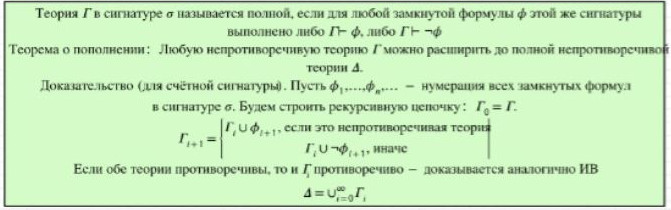
\includegraphics[width=13cm]{images/1.5_m1}

    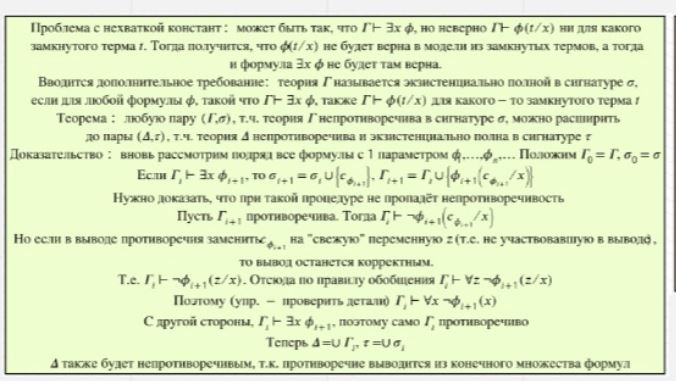
\includegraphics[width=13cm]{images/1.5_m2}

    
\includegraphics[width=12cm]{images/1.5_m3}

    
\includegraphics[width=12cm]{images/1.5_full}
\end{center}

\textbf{Лемма 9}.
Любую непротиворечивую теорию можно расширить до непротиворечивой, полной и экзистенциально полной теории.

Доказательство было приведено выше.

\subsection{Теорема Гёделя о полноте исчисления предикатов: построение модели из замкнутых термов у любого непротиворечивого, полного и экзистенциально полного множества.}

\textbf{Лемма 10}.

Любая непротиворечивая, полная, экзистенциально полная теория совместна, то есть имеет модель.
\begin{center}
    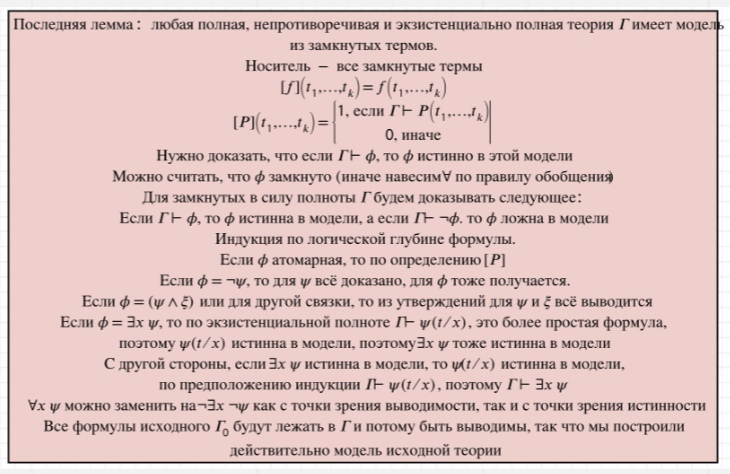
\includegraphics[width=12cm]{images/1.5_full2}    
\end{center}

\subsection{Представимость конечных последовательностей в арифметике при помощи $\beta$-функции Гёделя.}

\textbf{Лемма 1}:\\

$\forall n \quad \forall c \quad \exists b > c$ такое, что $b + 1,  2b + 1, \dotsc, nb + 1$ - взаимно просты.\\

Рассмотрим $b = n!$.

Тогда возьмем произвольные различные $k$ и $m$ от $1$ до $n$. $gcd(kb + 1, mb + 1) = d > 1 \Rightarrow (k - m)b$ делится на $d$.

Значит т.к. $b = n!$ и $k - m < n$, получаем, что любой простой делитель числа $(k - m)b$ должен быть строго меньше $n$.\\

У $d$ есть простой делитель $p < n$.

$mb + 1$ делится на $p$.

$mb + 1 - m\cdot n!$ делится на $p \Rightarrow d = 1$ 
\\

\textbf{Лемма 2.}\\

$\forall (x_1, \dotsc, x_n) \quad\exists a, b \quad \forall i : a \equiv x_i \quad mod (b_i + 1)$\\

\textbf{Док-во:}\\

Выберем по Лемме 1 $b > max\{x_i\}$.\\

Тогда нужное $a$ найдётся по китайской теореме об остатках: Если натуральные числа $a_1, \dotsc, a_n$  попарно взаимно просты, то для любых $r_1, \dotsc, r_n$ таких, что $0 \leq r_i < a_i$ при всех $i : 0, \dotsc, n$ найдется число, которое при делении на $a_i$ дает остаток $r_i$ при всех $i$. Более того, если найдутся два таких числа, то они будут сравнимы по модулю $a_1 \cdot \dotsc \cdot a_n$.\\

Положим $\beta(a, b, i) = a \quad mod (bi + 1)$

$\beta$ арифметична: $r = x \quad mod(q) \Leftrightarrow r < q$ и $\exists s: x = sq + r$.

\subsection{Арифметичность предикатов «n — степень шестёрки» и $n = 2^k$.}

\textbf{Определение:} Предикат $P: \N^k \to \{0,1\}$ называется \textit{арифметичным}, если он выразим в стандартной интерпретации арифметики $\langle \N, +, \cdot, = \rangle$. Функция $f: \mathbb{N}^k \rightarrow \mathbb{N}$ называется \textit{арифметичной}, если арифметичен предикат $P_{f}: \mathbb{N}^{k+1} \rightarrow \{0,1\}$, где $P_f(x,y) = 1 \lra f(x) = y$.
\\
\\
\textbf{Степень шестерки}
\\
Степень шестерки можно выразить с использованием квантора по конечному множеству\\
    $\exists D (x \in D \wedge \forall y \in D (y = 1 \vee (y \ \vdots \ 6 \wedge \frac{y}{6} \in D)))$ \\ У нас есть $x, \frac{x}{6}, \frac{x}{36}, \frac{x}{216}, ..., 1$. Этакий мешок с числами. И если в нем есть х, то есть и $\frac{x}{6}$ и т.д., а остановиться это все может только на единице. Соответственно, если x - не степень шестерки, то возникнет не единица, и оба условия будут нарушены.
    \\
    \\
    Через обычные предикаты эта функция выражается с помощью кодирования Смаллиана. Оно лучше применимо для описания конечных множеств. В чем суть:
    \\
    Берем и вводим предикат $S(a,b,x)$, которые отвечает следующим свойствам:
    \begin{itemize}
        \item [1] $\forall a,b\{x: S(a,b,x) = 1\}$ - конечно
        \item[2] Для любого конечного S найдутся такие a и b, что $S = \{x: S(a,b,x) = 1\}$
    \end{itemize}
    Теперь записанную нами формулу $\exists D .... x \in D....$ можно переписать следующим образом:\\
    $\exists a,\exists b (S(a,b,x) \wedge \forall y(S(a,b,y) \rightarrow (y = 1 \vee(y \ \vdots \ 6 \wedge \exists z(y = 6\cdot z \wedge S(a,b,z))))))$ \\
    Что поменялось? Заменили $\exists D$ на $\exists a, \exists b$. И $x \in D$ на $S(a,b,x)$, получили формулу первого порядка\\\\
\textbf{Степень двойки}\\
$x = 2^k $ можно выразить с использованием квантора по конечной последовательности\\
$\exists \{a_i\} (a_0 = 1 \wedge a_k = x \wedge \forall i \in [0;k-1] \ a_{i+1} = a\cdot a_i)$
\\
\\
Через обычные предикаты это выражается с использованием $\beta$-функции Гёделя. 
\\
Тут вводится арифметическая функция $\beta(a,b,i)$ со следующим свойством:
\begin{itemize}
    \item[] $\forall [x_0, ..., x_n]$ найдутся такие a,b, что $\forall i \in [0,n] \ x_i = \beta(a,b,i)$
\end{itemize}
Теперь в формуле, которая имеет вид $\exists \{x_i\} ......x_j......$ можно заменить на такую: $\exists a \exists b ......\beta(a,b,j)......$
\\
\\
Применим полученные знания к нашему предикату и получим:\\
$x = 2^k \Longleftrightarrow \exists a,b \ (\beta(a,b,0) = 1 \wedge \beta(a,b,k) = x \wedge \forall i \in [0,..., k-1] \ \beta(a,b,i+1) = 2\cdot \beta(a,b,i) $


\subsection{Множество замкнутых формул, истинных в $\mathbb N$, неперечислимо. Первая теорема Гёделя о неполноте.}

\textbf{Опр} Множество A $\subset \mathbb{N}^k$ называется \textit{арифметическим}, если существует арифметическая формула $\alpha$ с параметрами $x_1, . . . , x_k$, которая его представляет в следующем смысле: $<n_1, . . . , n_k>$ принадлежит множеству A тогда и только тогда, когда формула $\alpha$ истинна при значениях параметров $x_1 = n_1, . . . , x_k = n_k$.
\\
\\
Любое перечислимое множество арифметично
\\
\\
\textbf{Лемма1}\\
Всякое арифметическое множество лежит в классе $\Sigma_n$ или $\Pi_n$ для некоторого n (и, естественно, для всех больших n).
\\
$\blacktriangle$ Формулу, задающую арифметическое множество, приведём к предварённой нормальной форме (вынеся кванторы наружу). Ясно, что бескванторная часть задаёт разрешимое множество, поэтому исходное множество принадлежит какому-то из классов $\Sigma_n$ или $\Pi_n$. Можно и не использовать предварённой нормальной формы, а применить индукцию по длине формулы и сослаться на то, что пересечение, объединение и дополнение, а также проекция не выводят за пределы арифметической иерархии (объединения всех классов $\Sigma_n$ и $\Pi_n$). $\blacksquare$
\\
\\
Рассмотрим теперь множество T, элементами которого являются
все истинные арифметические формулы без параметров (точнее, их номера в какой-то вычислимой нумерации всех формул — это значит, что по формуле можно алгоритмически получить её номер и наоборот).
\\
\\
\textbf{Лемма2}\\ Любое арифметическое множество m-сводится к множеству T.\\
$\blacktriangle$ Пусть A — произвольное арифметическое множество. Пусть $\alpha$(x) — формула с одной переменной, которая выражает принадлежность множеству A. Это означает, что $\alpha$(n) истинно при тех и только тех n, которые принадлежат A.
Тогда вычислимая функция n $\rightarrow$ (номер формулы, которая является
результатом подстановки константы n в $\alpha$(x)) m-сводит A к T. $\blacksquare$
\\
\\
\textbf{ Первая теорема
Гёделя о неполноте}\\
Множество T арифметических истин неперечислимо.\\
$\blacktriangle$ Это следует из того, что если бы Т было перечислимо, оно было бы арифметично, что противоречит теореме Тарского $\blacksquare$ 
\\
\\
\textbf{Множество замкнутых формул, истинных в N, неперечислимо } \\
Если множество перечислимо, то оно лежит в арифметической иерархии, что противоречит теореме Тарского


\subsection{Теорема Тарского.}

\textbf{Теорема Тарского}\\
Истинность арифметической формулы нельзя выразить арифметическим выражением. То есть не существует формулы True(x), которая истинна тогда и только тогда, когда формула с номером х истинна. (Множество T не арифметично.)
\\
$\blacktriangle$ Если бы T было арифметическим, то оно лежало бы в некотором конкретном классе . Поскольку всякое арифметическое множество сводится к T, то все арифметические множества лежали бы в этом классе. Но мы знаем, что множества из более высоких классов иерархии тоже арифметичны, но в $\Sigma_n$ не лежат.$\blacksquare$
    
    \newpage
    \begin{center}
        \Huge\bfseries
        {Теория множеств.}
    \end{center}
    \addcontentsline{toc}{part}{Теория множеств.}
    \section{Определения}

\subsection{Множество, основные теоретико-множественные операции, упорядоченная пара, декартово произведение.}
\
\begin{enumerate}
    \item \textit{Множеством} называется произвольный набор (совокупность, класс, семейство) каких-либо объектов. Объекты, входящие во множество, называются его \textit{элементами}. Если объект $x$ является элементом множества $A$, то говорят, что $x$ принадлежит $A$, и пишут $x \in A$.
    \item Множество $A$ является \textit{подмножеством} множества $B$, если любой элемент множества $A$ также принадлежит множеству $B$. Обозначение: $A \subset B$.
    \item Множества $A$ и $B$ \textit{равны}, если одновременно $A \subset B$ и $B \subset A$. Обозначение: $A = B$.
    \item  Для задания \textit{упорядоченной пары} нужно задать неупорядоченную и первый элемент в ней. Например, по упрощённому определению Куратовского: $(a, b) = \{a, \{a, b\}\}$.
    \item \textit{Кортежем} длины 0 называется пустое множество. Если уже задан $T = (a_{1}, \ldots, a_{n})$ -- кортеж длины $n$, то $(a, a_{1}, \ldots, a_{n}) = \{a, \{a, T\}\}$ есть кортеж длины $n + 1$. Так можно получить ещё одно определение упорядоченной пары: $(a, b) = \{a, \{a, \{b, \{b, \emptyset\}\}\}\}$.
    \item \textit{Декартовым произведением} множеств $A$ и $B$ называется множество упорядоченных пар $A \times B = \{(a, b) \ | \ a \in A, b \in B\}$. \textit{Декартовой степенью} $A^n$ множества $A$ называется множество кортежей длины $n$ из элементов $A$.
\end{enumerate}

\begin{itemize}
    \item \textit{Объединением} $A$ и $B$ называется множество $A \cup B = \{x \ | \ x \in A \text{ или } x \in B\}$.
    \item \textit{Пересечением} $A$ и $B$ называется множество $A \cap B = \{x \ | \ x \in A \text{ и } x \in B\}$.
    \item \textit{Разностью} $A$ и $B$ называется множество $A \backslash B = \{x \ | \ x \in A \text{ и } x \not\in B\}$.
    \item \textit{Симметрической разностью} $A$ и $B$ называется множество $A \triangle B = (A \backslash B) \cup (B \backslash A)$.
    \item \textit{Дополнением} множества $A$ называется множество $A = \{x \ | \ x \not\in A\}$.
\end{itemize}

\subsection{Отображения и соответствия. Образ и прообраз. Инъекции, сюръекции, биекции. Композиция отображений. Возведение множества в степень множества.}

\begin{enumerate}
    \item \textit{Соответствием} между множествами $A$ и $B$ называют произвольное подмножество декартова произведения $F \subset A \times B$.
    \item \textit{Отображением} из множества $A$ в множество $B$ называется однозначное соответствие между $A$ и $B$, т. е. такое соответствие, что для любого $a \in A$ найдётся ровно одно $b \in B$, соответствующее $a$.
    \item Соответствие $F$ называется \textit{инъективным}, если для любых $a_1 \neq a_2$ множества $F(a_1)$ и $F(a_2)$ не пересекаются. Инъективное отображение называется \textit{инъекцией}.
    \item Соответствие $F$ называется \textit{сюръективным}, если любой элемент $B$ соответствует хотя бы одному элементу $A$, т. е. любой $b \in B$ лежит в $F(a)$ для некоторого $a \in A$. Сюръективное отображение называется \textit{сюръекцией}.
    \item \textit{Биекцией} называется отображение, являющееся одновременно инъекцией и сюръекцией.
    \item Пусть $F: A \rightarrow B$ -- соответствие, а $S \subset A$. \textit{Образ} $S$ -- это множество $F(S) = \bigcup_{s \in S} F(s) \subset B$.
    \item Пусть $F: A \rightarrow B$ -- соответствие, а $T \subset B$. \textit{Проообраз} $T$ -- это множество $F^{-1}(T) = \{a \ | \ F(a) \cap T \neq \emptyset\} \subset A$.
    \item Пусть $F: A \to B$ и $G: B \to C$ -- соответствия. Тогда их \textit{композицией} $G \circ F$ называется соответствие $H: A \to C$, определенное правилом: $c \in H(a)$ тогда и только тогда, когда найдется $b$, такое что одновременно $c \in G(b)$ и $b \in F(a)$.
    \item Пусть $A$ и $B$ -- два множества. Тогда множеством $B^A$ называется множество всех отображений из $A$ в $B$.
\end{enumerate}

\subsection{Равномощность. Счётные и континуальные множества.}

\begin{enumerate}
    \item Множества $A$ и $B$ назваются \textit{равномощными}, если существует биекция $A \to B$. Обозначение: $A \cong B$.
    \item Множество $A$ называется \textit{счетным}, если оно равномощно множеству $\N$.
    \item Множество $A$ называется \textit{континуальным}, если оно равномощно множеству $\R$.
\end{enumerate}

\subsection{Бинарные отношения. Рефлексивность, транзитивность, (анти)симметричность и т. д. Отношения эквивалентности и отношения порядка.}

\textbf{Определение:} \textit{Бинарным отношением} на множестве $A$ называется любое подмножество $R \subset A \times A$.

\begin{center}
    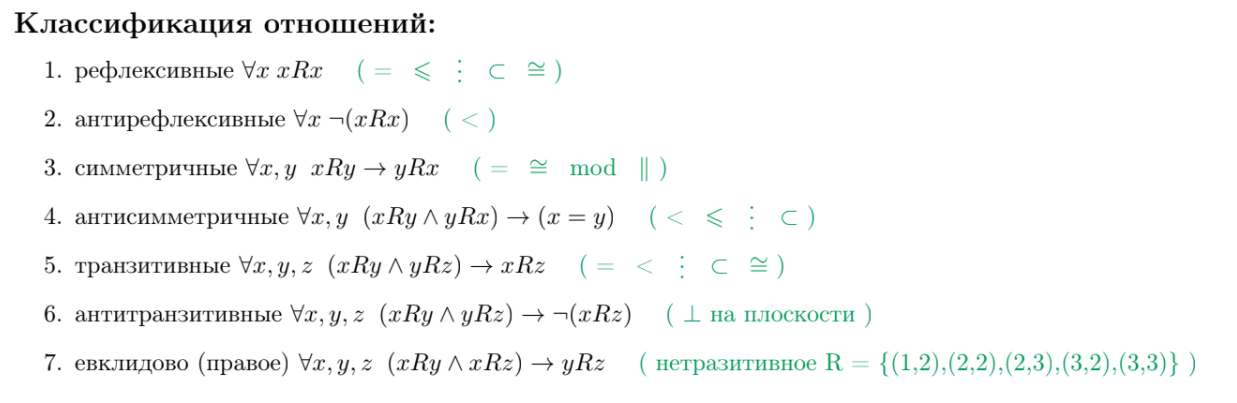
\includegraphics[width = 0.92\textwidth]{images/2 (определения)_m22.PNG}

    
\includegraphics[width = 0.93\textwidth]{images/2 (определения)_m23.PNG}
\end{center}

\subsection{Упорядоченное множество, линейно упорядоченное множество, фундированное множество, вполне упорядоченное множество.}

\textbf{Определение:} \textit{Упорядоченым множеством} называется пара $(A, \leq_A)$ -- множество и отношение порядка на нем.

\textbf{Определение:} Частично упорядоченное множество называется \textit{линейно упорядоченным}, если любые два элемента в нем сравнимы.

\textbf{Определение:} Частично упорядоченное называется \textit{фундированным}, если в любом его непустом подмножестве есть минимальный элемент.

\textbf{Пример}
\begin{itemize}
    \item [$\checkmark$] $\langle\mathbb{N}, \leq\rangle$, $\langle\mathbb{N} + \mathbb{N}, \leq\rangle$, $\langle\mathbb{N},|\rangle$ с заданным тривиально порядком -- фундированные.
    \item [$\times$] $\mathbb{Z}$, $[0,1]$ -- не фундированные.
\end{itemize}

\textbf{Определение:} Фундированное линейно упорядоченное множество называется \textit{вполне упорядоченными}, а соответствующий порядок -- полным.

\textbf{Пример}
\begin{itemize}
    \item [$\times$ ] Множество всех конечных слов из букв латинского алфавита.
    \item [$\times$ ] [0,1], $\langle \mathbb{N},|\rangle$.
    \item [$\checkmark$ ] $\mathbb{N}$.
\end{itemize}

\subsection{Цепи в упорядоченных множествах. Верхние и нижние грани, максимальные и минимальные, наибольшие и наименьшие элементы.}

\textbf{Определение:} Подмножество частично упорядоченного множества называется \textit{цепью}, если любые два его элемента сравнимы.

\textbf{Определение:} Элемент $a \in M$ называется \textit{минимальным}, если $b \leq a$ только при $b = a$. Элемент $a \in M$ называется \textit{наименьшим}, если $\forall b\in M: a \leq b$.
Аналогично вводятся понятия \textit{максимального} и \textit{наибольшего} элементов.

\textbf{Определение:} \textit{Верхней гранью} множества $A$ называется такой элемент $M$, что $\forall x \in A: \ x\leq M$.

\textbf{Определение:} \textit{Нижней гранью} множества $A$ называется такой элемент $m$, что $\forall x \in A: \ x\geq m$.

\subsection{Гомоморфизмы и изоморфизмы упорядоченных множеств.}

\textbf{Определение:} \textit{Гомоморфизмом упорядоченных множеств} называется функция $f:A\rightarrow B$, такая что
\begin{center}
    $x \leq_A y \lra f(x) \leq_B f(y)$.
\end{center}

\textbf{Определение:} \textit{Изоморфизмомом  упорядоченных множеств} называется  функция $f:A\rightarrow B$, являющаяся гомоморфизмом и биекцией.

\subsection{Сложение и умножение упорядоченных множеств.}


\includegraphics[width = 0.94\textwidth]{images/2 (определения)_m24.PNG}


\includegraphics[width = 0.94\textwidth]{images/2 (определения)_m25.PNG}

\subsection{Начальные отрезки вполне упорядоченных множеств.}
\textbf{Определение:} Пусть $S$ -- ВУМ. Подмножество $A \subset S$ называется \textit{начальным отрезком}, если $\forall x \forall y \left((x \leq y \land y \in A) \to x \in A \right)$.

\textbf{Примеры}
\begin{itemize}
    \item [$\checkmark$] $[0,a] = \{x \ | \ x\leq a\}$.
    \item [$\checkmark$] $[0,a) = \{x \ | \ x<a\}$.
    \item [$\checkmark$] Всё $S$.
\end{itemize}

\subsection{Предельные элементы вполне упорядоченных множеств.}

\textbf{Определение:} В любом ВУМ у любого элемента $a$, кроме максимального, есть единственный \textit{непосредственно следующий} за ним (элемент $a + 1$), т.е. такой $c > a$, что не существует такого $b$, что $a < b < c$.

\textbf{Определение:} \textit{Предельным элементом} ВУМ называется элемент, не являющийся непосредственно следующим ни для какого другого элемента.

\subsection{Порядковые типы $\omega, \omega^k, \omega^{\omega}, \epsilon_0$.}

\textbf{Определение:} Неформально \textit{ординалом} (порядковым числом или порядковым типом) называется
класс эквивалентности вполне упорядоченных множеств по отношению изоморфности. Формально ординалом называется транзитивное множество, каждый элемент которого также транзитивен.

Будем обозначать $0$ -- порядковый тип пустого множества, $1$ -- порядковый тип множества из одного элемента, $k$ -- порядковый тип линейного порядка на $k$-элементном множестве (такие ординалы называются конечными), $\omega$ -- порядковый тип множества натуральных чисел $\N$ со стандартным порядком.

Рассмотрим порядковый тип $\omega$. Следующим за ним будет $\omega + 1$, потом $\omega + 2, \ldots, \omega + \omega = \omega \cdot 2, \omega \cdot 2 + 1, \ldots, \omega \cdot 3, \ldots, \omega \cdot \omega = \omega^2$. Далее идут $\omega^2 + 1, \ldots, \omega^2 + \omega, \ldots, \omega^{2}\cdot 2, \ldots, \omega^3, \ldots, \omega^\omega, \ldots, \omega^{\omega + 1}, \ldots, \omega^{\omega^{\omega}}, \ldots, \epsilon_{0} = \omega^{\omega^{\omega^{\ldots}}}$($\omega$ раз).

$\epsilon_0$ -- минимальный ординал, такой что $\epsilon_0 = \omega^{\epsilon_0}$.

\subsection{Аксиома выбора.}

Пусть задано некоторое множество $A$. Тогда существует функция $\phi: 2^A \setminus \{A\} \rightarrow A$ такая, что $\forall S \subset A:\ \phi(S) \in S$.

\subsection{Базис Гамеля.}

Базис Гамеля в $\mathbb R$ над $\Q$ это такой набор действительных чисел, что любое другое действительное число представляется как конечная линейная комбинация элементов базиса с рациональными коэффициентами, при этом никакая нетривиальная конечная линейная комбинация элементов базиса с рациональными коэффициентами не равна $0$.
    \newpage
    \section{Простые утверждения}

\subsection{Основные тождества про теоретико-множественные операции, декартово произведение, возведение множества в степень множества.}

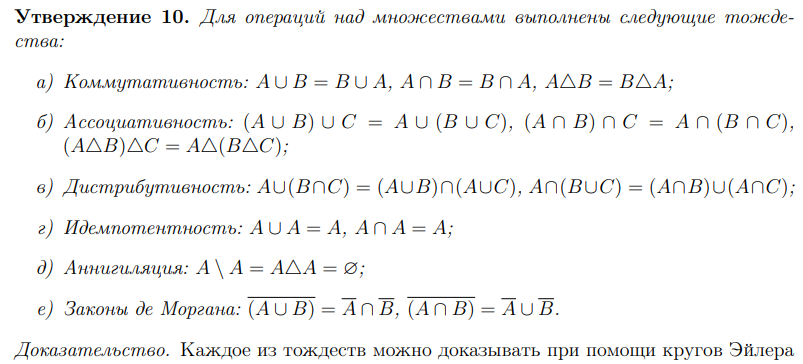
\includegraphics[width = 0.92\textwidth]{images/prop_10_sets.png}

\textbf{Определение:} Множества $A$ и $B$ эквивалентны, если для каждого элемента $A$ есть элемент $B$, задающий тот же кортеж, и наоборот. Будем обозначать такую эквивалентность как $A \sim B$.

\textbf{Cвойства:}
\begin{enumerate}
     \item $A^n \sim A\times A\ldots \times A$ -- по определению.
     \item $(A\times B)\times C \sim A \times( B \times C )$:\\
     $A \times B = \{(a,b): \ a \in A, b\in B\}; \\ (A \times B)\times C = \{((a,b),c): \ a \in A, b\in B, c \in C\} \sim \{(a,(b,c)): \ a \in A, b\in B, c \in C\} = A\times (B \times C)$.
     \item $A \times \{\emptyset\} \sim A$.
     \item $A^{n+k} \sim (\underbrace{A\times A \times \ldots \times A}_{n})(\underbrace{A\times A \times \ldots \times A}_{k}) \sim \underbrace{A\times A \times \ldots \times A}_{n+k} \sim A^n \times A^k$.
     \item $(A^n)^m \sim A^{nm}$.
\end{enumerate}

\textbf{Cвойства:}
\begin{enumerate}
    \item $(A \times B)^C \sim A^C \times B^C$.
    \item $A^{B \cup C} \sim A^B \times A^C$, если $B$ и $C$ не пересекаются.
    \item $(A^B)^C \sim A^{B \times C}$.
\end{enumerate}

\textit{Доказательство:} 
\begin{enumerate}
    \item Пусть $F \in (A \times B)^C$. Это значит, что $F : C \to A \times B$. То есть каждому элементу $c \in C$ сопоставлена некоторая пара $(a, b) \in A \times B$. Вместо этого ему можно сопоставить отдельно элементы $a \in A$ и $b \in B$. Получится два отображения, первое отображает $c$ в $a$, а второе -- $c$ в $b$, то есть пара отображений $(F_1, F_2) \in A^C \times B^C$.
    \item Вторая эквивалентность означает, что определить функцию на несвязном объединении двух множеств это то же самое, что определить её на каждом из этих множеств по отдельности.
    \item Третья эквивалентность означает, что функция двух аргументов есть то же самое, что отображение первого аргумента в функцию, зависящую от второго аргумента.
\end{enumerate}

\subsection{Равномощность — отношение эквивалентности.}

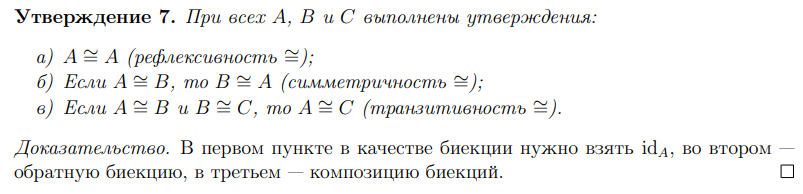
\includegraphics[width = 0.92\textwidth]{images/equiv_sets.png}

\subsection{Объединение и декартово произведение счётных множеств счётны.}

\textbf{Утверждение:} Пусть $A$ -- счётное множество, а $b \not\in A$. Тогда $A \cup \{b\}$ тоже счётно.

\textit{Доказательство:} Формально, пусть $\alpha: \N \to A$ -- биекция. Тогда определим биекцию $\beta: \N \to (A \cup \{b\})$ так: $\beta(0) = b$ и $\beta(n) = \alpha(n - 1)$ для $n > 0$.

\textbf{Утверждение:} Если $A$ счётно, а $B$ конечно, то $A \cup B$ тоже счётно.

\textbf{Утверждение:} Если $A$ и $B$ суть счётные множества, то $A \cup B$ тоже счётно.

\textit{Доказательство:} Ясно, что $A \cup B = A \cup (B \setminus A)$. Если множество $B \setminus A$ конечно, то утверждение следует из предыдущего. Иначе $B \setminus A$ счётно.

Таким образом, утверждение достаточно доказать для непересекающихся $A$ и $B$. В этом случае пусть $\alpha: \N \to A$ и $\beta : \N \to B$ суть биекции. Тогда построим биекцию $\gamma : \N \to A \cup B$ по правилу: $\gamma(2k) = \alpha(k)$, а $\gamma(2k + 1) = \beta(k)$.
    
\textbf{Утверждение:} Декартово произведение двух счётных множеств $A \times B$ cчётно.

\textit{Доказательство:} В самом деле, по определению декартово произведение есть множество всех упорядоченных пар вида $\langle a, b \rangle$, в которых $a \in A$ и $b \in B$. Разделим пары на группы, объединив пары с одинаковой первой компонентой (каждая группа имеет вид $\{a\}\times B$ для какого-то $a \in A$). Тогда каждая группа счётна, поскольку находится во взаимно однозначном соответствии с $B$ (пара определяется своим вторым элементом), и групп столько же, сколько элементов в $A$, то есть счётное число.

\subsection{В любом бесконечном множестве найдётся счётное подмножество.}
Так как $A$ бесконечно, в нем существует элемент $a_0$, причем $A\backslash{a_0}$ также бесконечно. Значит, в нем найдется $a_1$. Продолжая набирать элементы, получим множество $A_1 = \{a_0, a_1,\ldots\}$, $A_1 \subset A$.

\subsection{Несчётность множества точек на отрезке.}

Ясно, что любые два отрезка равномощны, так что рассмотрим отрезок $[0, 1]$. Докажем несчётность интервала $(0, 1)$, из чего будет несчётность отрезка.

Рассмотрим биекцию $f(x) = \tg(\pi(x - \frac{1}{2}))$.

\subsection{Нефундированность прямого лексикографического порядка на конечных словах.}
Нефундированность следует из существования бесконечно убывающей цепочки. Например, можно рассмотреть последовательность: $b > ab > aab > \ldots$.

\subsection{Любой начальный отрезок вполне упорядоченного множества, отличный от всего множества, представляется в виде $[0, a)$.}

\textbf{Теорема:} Если $S$ -- ВУМ, $A$ -- начальный отрезок $S$, $A \neq S$, то $A = [0, y)$.

\begin{proof}
    Рассмотрим $\overline{A} = S \backslash A$. Так как $\overline{A} \neq \varnothing$, то по свойству фундированности $\exists y =$ min$\overline{A},$ тогда покажем, что $A = [0, y)$. $[0, y) \subset A,$ так как если $x \in [0, y)$ и $x \notin A,$ то $x < y$ и $x \in \overline{A} \Rightarrow y \neq$ min$\overline{A}$, противоречие. $A \subset [0, y),$ так как если $x \in A$ и $x \notin [0, y),$ то (поскольку это ЛУМ) $x \geqslant y \Rightarrow$ (по определению начального отрезка) получаем, что $y \in A$ противоречие.
\end{proof}

\subsection{Вполне упорядоченное множество неизоморфно своему начальному отрезку вида
[0, a) (вывод из леммы о монотонной функции).}
\begin{center}
    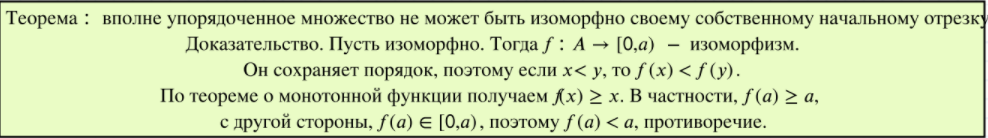
\includegraphics[width = 17cm]{images/2 (определения)_m211.PNG}
\end{center}

\subsection{Сумма и произведение фундированных множеств фундированы, вполне упорядоченных — вполне упорядочены.}

\begin{center}
    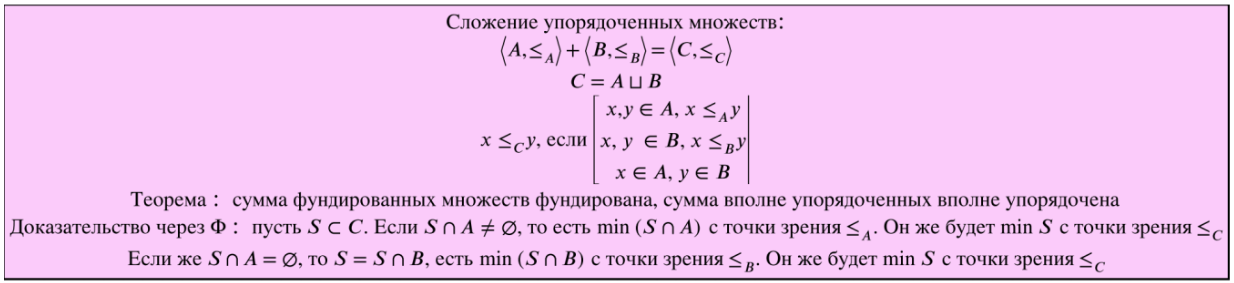
\includegraphics[width = 17cm]{images/sum_fund.png}
\end{center}
\begin{center}
    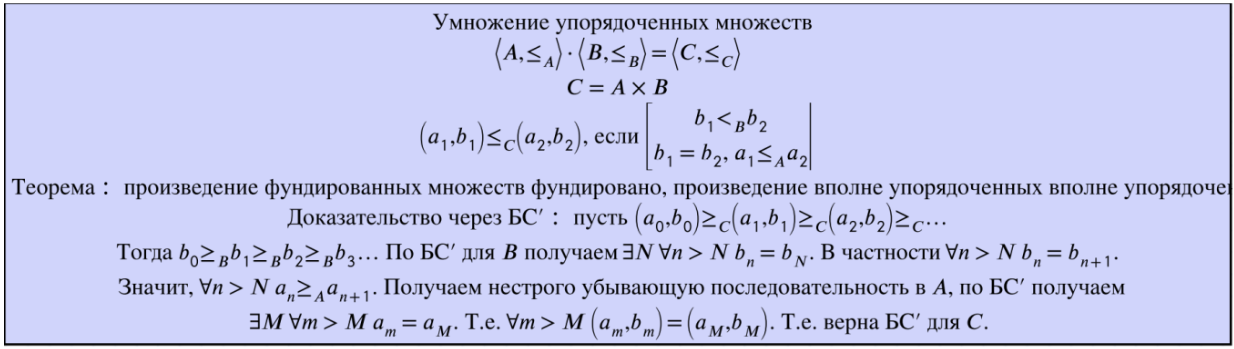
\includegraphics[width = 17cm]{images/cdot_fund.png}
\end{center}

\subsection{Свойства сложения и умножения вполне упорядоченных множеств: ассоциативность, некоммутативность, (не)дистрибутивность, (не)монотонность.}

Верны ассоциативность и правая дистрибутивность: $A\cdot(B + C) \simeq A\cdot B + A\cdot C$. Коммутативность и левая дистрибутивность неверны: $1+\omega = \omega \neq \omega+1$, $2 \cdot \omega = \omega \neq \omega \cdot 2$, $(1 + 1) \cdot \omega = \omega \neq 1 \cdot \omega + 1 \cdot \omega$.

Условие монотонности звучит так: если $A < B (A \lesssim B)$, то верно ли, что для всех $C$ истинно $A+C < B+C$, $C + A < C + B$, $A \cdot C < B \cdot C$, $C \cdot A < C \cdot B$ (то же для $\lesssim$ вместо $<$)?

При $A < B$ верно $C + A < C + B$, $A + C \lesssim B + C$, $C \cdot A < C \cdot B$ (при непустом $C$), $A \cdot C \lesssim B \cdot C$. При $A \lesssim B$ все неравенства верны с $\lesssim$.

\subsection{Сравнимость любых двух множеств по мощности (вывод из теоремы Цермело и свойств вполне упорядоченных множеств).}
\begin{center}
    
\includegraphics[width = 17cm]{images/2 (определения)_mm1.PNG}\\    
\end{center}
\textbf{Сравнимость любых двух множеств по мощности}\\
По теореме Цермело для любого множества существует равномощное ему ВУМ. Пусть даны $A, B$, а $A', B'$ соответствующие им ВУМы, удовлетворяющие теореме Цермело. Тогда из теоремы о сравнимости ВУМов $A'$ и $B'$ сравнимы по мощности, значит, $А$ и $В$ также сравнимы по мощности.

\subsection{Теорема о структуре: любой элемент вполне упорядоченного множества представляется как сумма предельного и конечного.}

\textbf{Теорема:} Для любого элемента $a$ вполне упорядоченного множества найдётся предельный элемент $b$ и натуральное число $k$, такое что $a = \underbrace{S(S(\ldots (S}_{k \text{ раз }}(b))\ldots))$.

\textit{Доказательство:} Нужно брать непосредственно предыдущий, пока не придём к предельному. Прийти обязаны, иначе будет бесконечно убывающая последовательность.
    \newpage
    \section{№2 Не абелевы группы}

\begin{reminder}
    Группа $(G, \cdot)$
    \begin{itemize}
        \item $(G1): x \cdot (y \cdot z) = (x \cdot y) \cdot z$ 
        \item $(G2): \exists c \in G \  \forall x: \ x \cdot e = e \cdot x = x$ 
        \item $(G3): \forall x \in G \  \exists x^{-1}: \ x \cdot x^{-1} = x^{-1} \cdot x = e$ 
        \item Абелевы группы: $x \cdot y = y \cdot x$
        \end{itemize}

\end{reminder}

\subsection{Группы биекций}

\begin{itemize}
    \item Тотальная функция: $f: A \ra B$
    \item Инъекция $\Lra f(x_1) = f(x_2) \Ra x_1 = x_2$
    \item Сюръекций $\Lra \forall y \in B \  \exists x \in A: \ f(x) = y$
    \item Биекция $\Lra$ инъекция и сюръекция
\end{itemize}

\subsection{Композиция функций}

\begin{definition}
    Пусть заданы функции $f, g: A \ra A$. Тогда их композицией будет:

    $(f \circ g)(x) = f(g(x))$
\end{definition}


\begin{example}
    $(S(x), +)$ --- группа.

    Где, $X$ --- множество, $S(x)$ --- биекция $X \ra X$.
\end{example}


% Пример: $(S(x),\  +)$ -- группа \\
% X -- множество \\
% S(x) -- биекция $X \rightarrow X$ \\


% Композиция \\
\begin{note}
    \[\big( (f \comp g) \comp h \big)(x) = \big( f \comp (g \comp h) \big)(x) \Ra\]
    \[\Ra \bigl( \big(g(h(x))\big) \bigl)\]
    \[\id : \ x \raone x\]
\end{note}

% $id: x \rightarrow x$ \\

Обратная функция --- просто биекция в другую сторону

\begin{example}[Не абелевой группы]
    \[f: \  x \raone x + 1\]
    \[g: \  x \raone -x\]
    \[(f \comp g)(x) = -x + 1\]
    \[(g \comp f)(x) = -x - 1\]
    Т.е. порядок имеет значение.
\end{example}
% Пример: \\
% $f: x \rightarrow x + 1$ \\
% $g: x \rightarrow -x$ \\
% \[(f \circ g)(x) = -x + 1\] 
% \[(g \circ f)(x) = -x - 1\], т.е. не равны \\

\newpage
\subsection{Перестановки}

\begin{definition}
    $X = \left \{1, 2, \dots n \right \}$ --- множество $n$ элементов.

    $S_n = S(x)$ --- группа перестановок степени $n$.
\end{definition}

\begin{enumerate}
    \item[I.] \ul{Размещение} из $n$ по $n$. 
    
    34512
    \item[II.] \ul{Табличный}
    
    \[
        \Pi = 
        \begin{pmatrix}
            1 2 3 4 5 \\
            3 4 5 1 2
        \end{pmatrix}
        \]
        
        $\Pi (1) = 3$.
        
        \[
        \sigma = 
        \begin{pmatrix}
            1 2 3 4 5 \\
            2 1 3 4 5
        \end{pmatrix}
        \]
        
        \[
        (\Pi \  \circ \  \sigma)  = 
        \begin{pmatrix}
            1 2 3 4 5 \\
            $\st{21345}$ \\
            4 3 5 1 2
        \end{pmatrix}
        \]
    \item[III.] \ul{С помощью графа}. Входящие и исходящие степени равны по 1, так как является биекцией.

    \[\Pi = (13524) = (52413)\]
    \[\sigma = (12)\] Bключая циклы длины 1 (просто их не пишем).
    
    \[(\Pi \circ \sigma) = (14)(23)\]
    
\end{enumerate}

% 1. Размещение из n по n \\
% $2451$ \\

% 2. Табличный \\
% \[
% \Pi = 
% \begin{pmatrix}
%     1 2 3 4 5 \\
%     3 4 5 1 2
% \end{pmatrix}
% \]

% $\Pi (1) = 3$

% \[
% \sigma = 
% \begin{pmatrix}
%     1 2 3 4 5 \\
%     2 1 3 4 5
% \end{pmatrix}
% \]

% \[
% (\Pi \  \circ \  \sigma)  = 
% \begin{pmatrix}
%     1 2 3 4 5 \\
%     2 1 3 4 5 \\
%     4 3 5 1 2
% \end{pmatrix}
% \], и вычеркнем центральную линию.

% 3. С помощью графа. Входящие и исходящие степени равны по 1, т.к. является биекцией.
% \[\Pi = (13524) = (52413)\]
% \[\sigma = (12), \] исключая циклы длины 1 (просто их не пишем).

% \[(\Pi \circ \sigma) = (14)(23)\]

% \subsection{Продолжение не абелевых групп}

\subsection{Общие свойства групповых операций}

\begin{enumerate}
    \item \ul{Закон сокращения}:
    \[\forall a \in G: \  x = y \Leftrightarrow ax = ay \Leftrightarrow xa = ya\]
    \[a^{-1}(ax) = (a^{-1}a)x = ex = x\]

    \item \ul{Формула обратного произведения}:
    \[(xy)^{-1} = y ^ {-1} \cdot x ^{-1}\]
    \[(xy)(y^{-1}x^{-1}) = x(y y^{-1}) x^ {-1} = xex^{-1} = x x^{-1} = e\]
    Проверка, что обратный единственный: \\
    \[C = x u = xv\] и получаем желаемое.
\end{enumerate}

% 1. Закон сокращения: \\
% \[\forall a \in G \  x = y \Leftrightarrow ax = ay \Leftrightarrow xa = ya\]
% \[a^{-1}(ax) = (a^{-1}a)x = ex = x\]

% 2. Формула обратного произведения: \\
% \[(xy)^{-1} = y ^ {-1} \cdot x ^{-1}\]
% \[(xy)(y^{-1}x^{-1}) = x(y y^{-1}) x^ {-1} = xex^{-1} = x x^{-1} = e\]
% Проверка, что обратный единственный: \\
% \[C = x u = xv,\] и получаем желаемое.

\subsection{Подгруппы}

\begin{definition}
    Подгруппа $H$ группы $G$: $H \subseteq G$ ($H < G$) (групповая операция та же самая).
\end{definition}

\begin{example}
    $3 \mathbb{Z}  = \left\{ x \mid x = 3y,\  y \in \mathbb{Z} \right\}$
\end{example}

\begin{definition}
    $GL(\mathbb{R}, n)$ --- общая группа линейных преобразований.
\end{definition}


Проверка, что элементы принадлежит группе:
\begin{itemize}
    \item[\text{$\left. 1 \right)$}] $e_G \in H: \begin{cases} e_H \cdot h = h, \\ e_G \cdot h = h \end{cases} \Ra e_H = e_G$
    \item[\text{$\left. 2 \right)$}] $x \in H \Ra x ^ {-1} \in H: \begin{cases} x_H^{-1} x = e, \\ x_G^{-1} x = e \end{cases} \Ra x_H^{-1} = x_G^{-1}$
    \item[\text{$\left. 3 \right)$}] $x, y \in H, \  x \cdot y \in H$
\end{itemize}

\begin{reminder}
    Вычеты --- $\bar{n} \ZZ \quad \left[a \right]_n = \left\{ x: x = a + z, z \in \bar n \ZZ \right\}$ ($H < G, \ g \in G$)
\end{reminder}

\begin{definition}
    ~

    Смежный (левый) класс --- $gH = \left\{x \mid x = gh, h \in H\right\}$,
    
    Смежынй (правый) класс --- $Hg = \left\{x \mid x = hg, h \in H\right\}$
\end{definition}

\begin{lemma}
    Смежные классы не пересекаются или совпадают.
\end{lemma}
\begin{proof}
    \begin{gather}
        z \in xH \  \land \  yH \quad z = x h_1 = y h_2, \quad h_1, h_2 \in H \\
        \begin{cases} x = y(h_2h_1^{-1}) \in yH, \quad xH \subseteq yH, \\
        xh_1 = y (h_2h_1^{-1}h_1) \in yH, \quad yH \subseteq xH \end{cases} \Ra xH = yH
    \end{gather}
\end{proof}

\subsection{Порядок группы}

\begin{definition}
    $|H| < \infty$ --- порядок группы.
\end{definition}

\[\Rightarrow |gH| = |H|\]
\[\alpha: H \ra gH\]
\[\alpha(h) = gH\]

\[gh_1 = gh_2 \Rightarrow h_1 = h_2\]

\begin{definition}
    $(G: H)$ --- индекс подгруппы (число смежных классов).
\end{definition}

\begin{theorem}[Лагранж]
    $|G| = |H| \cdot (G: H)$
\end{theorem}

\begin{itemize}
    \item[$1^{0}$] Порядок подгруппы делит порядок группы.
    \item[$2^{0}$] $|G| = p$ --- простое. В $G$ нет совместных подгрупп $\left\{ e \right\}, G$ --- несобственные.
    \item[$3^{0}$] $|G| = p$ --- простое, то $G$ -- абелева.
\end{itemize}

\begin{definition}
    $\langle g \rangle$ --- наименьшая подгруппа, содержащая g.
\end{definition}

\[\langle g \rangle = \left\{ e = g^0, g^1, g^2, \dots, g^{-1}, g^{-2} \right\}\]
\[\forall g: \ \langle g \rangle < G, \ |G| = p \Rightarrow \langle g \rangle = G\]

\begin{definition}
    Порядок элементов в группе --- $\ord g = |\langle g \rangle| \Leftrightarrow $ наименьшее $k: \  g^k = e$

\end{definition}

\begin{example}
    Рассмотрим группу: $(\ZZ_n, +)$
    \[\langle a \rangle = {\left [ ka \right ]}_n\]
    \[\ord a = \min k: ka \equiv 0 \mod n = \frac{\lcm (a, n)}{a} = \frac{n}{\gcdru (a, n)} \Ra\]
    \[\Ra \gcdru (a, n) \cdot \lcm (a, n) = a \cdot n\]
\end{example}


% $\langle a \rangle = {\left [ ka \right ]}_n$

% $\ord a = \min l: ka \equiv 0 \mod n = \frac{\lcm (a, n)}{a}$

$|\langle d \rangle| = \frac{n}{d}$

$|(\ZZ^{\text{*}}_n, \cdot)| = \phi (n) $ --- функция Эйлера.

\begin{theorem}[\text{Эйлер}]
    \[\gcdru(a, n) = 1 \Ra a^{\phi (n)} \equiv 1 \mod n\]
    \[k \cdot \ord a = \phi(n)\]
    \[a ^ {k \ord a} = (a ^ {\ord a})^k = 1 ^ k = 1\]
\end{theorem}

\begin{theorem}[\text{Малая теорема Ферма}]
    Если $p$ --- простое, то:
    \[a \not \equiv 0 \mod p \Ra a^{p - 1} \equiv 1 \mod p\]
\end{theorem}


    \newpage
    \begin{center}
        \Huge\bfseries
        {Вычислимость.}
    \end{center}
    \addcontentsline{toc}{part}{Вычислимость.}
    \section{Определения}

\subsection{Машина Тьюринга.}

\textbf{Определение: } Формальное определние \textit{машины Тьюринга} -- это кортеж ($\Sigma, \Gamma, Q, q_1, q_a, q_r, \delta$), где
\begin{itemize}
    \item[$\Sigma$] -- конечное непустое множество -- входной алфавит, типично $\{0,1\}$.
    \item[$\Gamma$] -- конечное непустое множество, включающее в себя $\Sigma$, как подмножество, а также, по меньшей мере, еще пустой символ (бланк, пробел) -- ленточный алфавит.
    \item[$Q$] -- конечное множество, не пересекающееся с $\Gamma$ -- множество внутренних состояний.
    \item[$q_1$]$\in Q$ -- начальное состояние.
    \item[$q_a$]$\in Q$ -- принимающее состояние.
    \item[$q_r$]$\in Q$ -- отвергающее состояние.
    \item[$\delta$] -- функция перехода. $\delta: Q\times\Gamma \rightarrow Q\times\Gamma \times\{L, R, N\}$, где L -- перемещение влево, R -- вправо, N -- никуда.
\end{itemize}

Для задач с текстовым или числовым ответом вместо $q_r, q_a$ рассматривают одно $q_0$.

\textbf{Определение: } \textit{Конфигурация машины Тьюринга} -- данные о содержимом ленты, положении указателя и состоянии упавляющего блока.

Начальная конфигурация: на ленте написан вход, машина в состоянии $q$, указывает на первый символ входа. У каждой конфигурации есть однозначно опредляемая следующая. Если состояние завершающее, конфигурация уже не меняется. Иначе производится замена символа, состояния и положения головки.

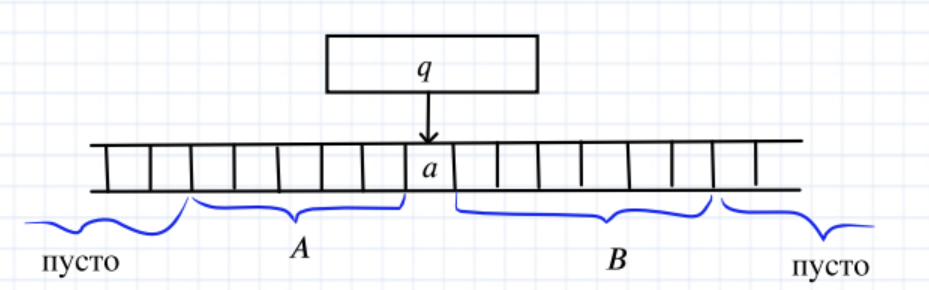
\includegraphics{images/3 (определения)_m31.PNG}

AqaB

\textit{Вычислением на машине Тьюринга} называется последовательность конфигураций, каждая из которых непосредственно следует из предыдущей по правилам этой машины.\\

\textbf{Пример смены конфигураций}

\begin{center}
    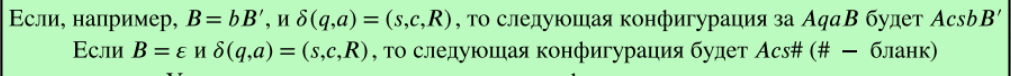
\includegraphics[width =17cm]{images/3 (определения)_mmm1.PNG}
\end{center}

q,s -- состояния

\subsection{Вычислимая функция.}

\textbf{Определение: } Функция $f: \{0,1\}^* \rightarrow \{0,1\}^*$ называется \textit{вычислимой}, если для некоторой машины Тьюринга выполнено:
\begin{itemize}
    \item[1] Если $f(x)$ определена, то существует вычисление, которое начинается с $q_{1}x$ и заканчивается $q_0f(x)$.
    \item[2] Если $f(x)$ не определена, то машина Тьюринга не остановится.
\end{itemize}

\textbf{Примеры}

\begin{center}
    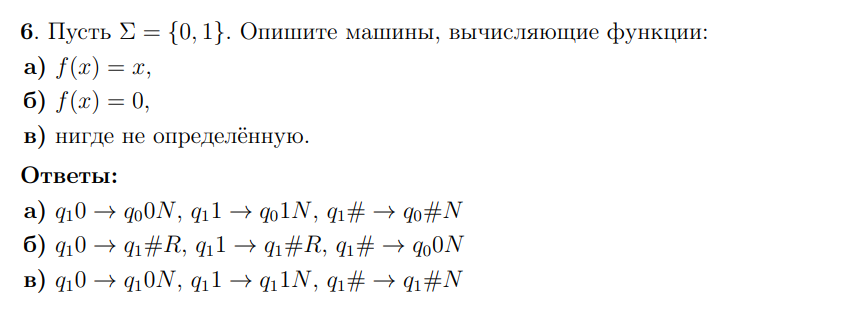
\includegraphics[width=15cm]{images/mt_1_def.png}
\end{center}

\subsection{Разрешимое множество.}

\textbf{Определение: } Множество $A \subset \{0,1\}^*$ называется \textit{разрешимым}, если для некоторой машины Тьюринга выполнено:
\begin{itemize}
    \item[1] Если $x \in A$, то существует вычисление на этой машине, которое начинается с $q_1x$ и заканчивается $q_a$.
    \item[2] Если $x \in \overline{A}$, то существует вычисление на этой машине, которое начинается с $q_1x$ и заканчивается $q_r$.
\end{itemize}

\subsection{Перечислимое множество.}

Будем рассматривать машину, у которой вместо завершающих состояний есть команды печати в поток вывода: печать 0, печать пробела. Результатом работы такой машины будет конечная или бесконечноая цепочка слов, разделенных пробелами.

\textbf{Определение: } Множество называется \textit{перечислимым}, если существует печатающая машина, такая что:
\begin{itemize}
    \item[] Если $x \in A$, то х встречается в потоке вывода.
    \item[] Если $x \not\in A$, то х не встречается в потоке вывода.
\end{itemize}

\textbf{Примеры}
\begin{itemize}
    \item [$\checkmark$] Пустое множество является перечислимым.
    \item [$\checkmark$] Область значений/Область определения любой вычислимой функции -- перечислимое множество.
    \item [$\times$] $\{n | U(n, x)$ определено при всех x$\}$ -- неперечислимо.
\end{itemize}

\subsection{Универсальная машина Тьюринга.}

\textbf{Определение: } \textit{Универсальная машина Тьюринга} -- это некоторая машина, которая получает на вход описание другой машины и вход для нее, а возвращает результат ее работы.
\[U(\langle M \rangle, x) = M(x).\]

\subsection{Универсальная вычислимая функция.}

\textbf{Определение: } Функция $u:\{0,1\}^* \times \{0,1\}^* \rightarrow \{0,1\}^*$ называется \textit{универсальной вычислимой функцией}, если:
\begin{itemize}
    \item[1] $u$ вычислима, как функция от двух аргументов.
    \item[2] Если $f:\{0,1\}^* \rightarrow \{0,1\}^* $ -- вычислимая функция одного аргумента, то $\exists p \forall x \ u(p,x) = f(x)$.
\end{itemize}

\subsection{Главная универсальная вычислимая функция.}

\textbf{Определение: } $U:\mathbb{N}\times\mathbb{N} \rightarrow \mathbb{N}$ -- \textit{главная универсальная вычислимая функция}, если
\begin{itemize}
    \item[1] $U$ вычислима.
    \item[2] $U$ универсальна, т.е. для любой вычислимой $f:\mathbb{N} \rightarrow \mathbb{N} $ найдется $p$ такое, что $\forall x f(x) = U(p,x)$ (говорят, что $p$ -- это номер функции $f$).
    \item[3] $U$ главная, т.е. для любой вычислимой $V: \mathbb{N}\times\mathbb{N} \rightarrow \mathbb{N}$ найдется всюду определенная вычислимая $s:\mathbb{N} \rightarrow \mathbb{N}$, такая что $\forall p \ \forall x \ V(p,x) = U(s(p),x)$.
\end{itemize}
Интуитивный смысл: $U$ -- универсальный компилятор, $V$ -- какой-то вычислимый. Первый аргумент $V$ -- \" \ программа\" \ , второй -- \" \ данные\" \ , $s$ -- \" \ автоматический траснлятор\" \ , переделывающие программу для $V$ в программу для $U$.

\subsection{$m$-сводимость.}

\textbf{Определение: } Говорят, что $A$ \textit{m-сводится} к $B$, если существует всюду определенная вычислимая функция $f:\mathbb{N} \rightarrow \mathbb{N}$, такая что $x \in A \lra f(x) \in B$. Обозначение: $A\leq_m B$.

\subsection{Арифметическая иерархия.}

\textbf{Определение: } Говорят, что множество $A $ принадлежит классу $\Sigma_n$, если существует такое разрешимое множество $R \in \mathbb{N}^{k+1}$, что
$$x \in A \lra \exists y_1 \ \forall y_2 \ \exists y_3 \ldots. \mathcal{Q} y_n [(x, y_1,\ldots,y_k) \in R].$$ 

Аналогично, говорят, что $A$ принадлежит классу $\Pi_n$, если существует такое разрешимое множество $R \in \mathbb{N}^{k+1}$, что
$$x \in A \lra \forall y_1 \ \exists y_2 \ \forall y_3 \ldots. \mathcal{Q} y_n [(x, y_1,\ldots,y_k) \in R].$$

Согласно этому определению, $\Sigma_0 = \Pi_0$ (классы $\Sigma_0$ и $\Pi_0$ совпадают с классом всех разрешимых множеств).

$\Sigma_1$ -- перечислимые, $\Pi_1$ -- коперечислимые

$\blacktriangle \ $S перечислимо $\lra$ для некоторого разрешимого R верно ($x \in S \lra \exists y \ (x,y) \in R$), Q коперечислимо $\lra$ для некоторого разрешимого R верно ($x \in S \lra \forall y \ (x,y) \in R$).

\textbf{Примеры}
\begin{itemize}
    \item[1] $T$ -- множество всюду определенных функций.
    
    $p \in T \lra \forall n \exists k (U(p,n)$ останавливается за $k$ шагов) -- разрешимое свойство $\Rightarrow T \in \Pi_2$.
    
    \item[2] $FD$ -- множество функций с конечной областью определения.
    
    $p \in FD \Leftrightarrow \exists N \forall n \ \forall k  (n > N \Rightarrow U(p,n)$ останавливается за k шагов) -- разрешимое свойство $\Rightarrow FD \in \Sigma_2$.
\end{itemize}

\subsection{$\lambda$-термы, $\alpha$-конверсии, $\beta$-редукции, нормальная форма.}

\textbf{Определение: } \textit{$\lambda$-терм} строится по индукции:
\begin{itemize}
    \item[1] Переменная является $\lambda$-термом.
    \item[2](Операция аппликации): Если M и N суть лямбда-термы, то (MN) - тоже лямбда-терм.
    
    Смысл: в функцию M вместо переменное подставляем N.
    \item[3](Операция $\lambda$-абстракции): Если M - терм, а x - переменная, то ($\lambda x.M$) - тоже терм.
    Смысл: выражение M теперь рассматривается как функция от х.
\end{itemize}

\textbf{Определение: } \textit{$\alpha$-конверсия} -- это замена связаной переменной. $\lambda x.M \rightarrow \lambda z.M(z/x)$

\textbf{Ограничение: не должно возникать конфликтов имен. Переменные из М не должны попадать под действие $\lambda$-квантора.}\\

\textbf{Пример}
\begin{itemize}
    \item [$\checkmark$] $\lambda x.xy \rightarrow \lambda z.zy$ -- так можно.
    \item [$\checkmark$] $\lambda x.xy(\lambda x.xy) \rightarrow \lambda z.zy(\lambda x.xy)$ -- и так можно.
    \item[$\times$] $\lambda x.xy \rightarrow \lambda y.yy$ -- а вот так нельзя.
    \item[$\times$] $\lambda x.x(\lambda y.xy) \rightarrow \lambda y.y(\lambda y.yy)$ -- и так тоже нельзя! Тут переменная, полученнная после замены, попала под воздействие уже имеющегося квантора.
\end{itemize}

\textbf{Определение: } \textit{$\beta$-редукция} -- это замена аргумента функции на какое-то значение. $(\lambda x.M)N \rightarrow M(N/x)$

\textbf{Ограничение: не должно возникать конфликтов имен. В N не должно быть переменных, по которым стоят $\lambda$-кванторы в М}\\

\textbf{Пример}
\begin{itemize}
    \item[$\checkmark$] sin x при x = 2 равен $\sin 2$.
    \item[$\times $] $(\lambda x.(x \lambda y.xy))y \rightarrow y\lambda y.yy$ -- так нельзя.
\end{itemize}

\textbf{Определение: } Говорят, что терм M находится в \textit{нормальной форме}, если к нему нельзя применить $\beta$-редукцию даже после нескольких $\alpha$-конверсий\\ Говорят, что N - нормальная форма M, если M = N и N находится в нормальной форме.

Не у всех термов есть нормальная форма.\\

\textbf{Пример}

$\Omega = (\lambda x.xx)(\lambda x.xx)$

\subsection{Нумералы Чёрча.}

\textbf{Определение: } 

Формально, число $k$ соответствует преобразованию функции $f$ в ее k-ую итерацию:

\begin{center}
    $\overline{0} = \lambda fx.x$
    
    $\overline{1} = \lambda fx.fx$
    
    $\overline{2} = \lambda fx.f(fx)$
    
    $\dots$
    
    $\overline{n} = \lambda fx. f(f\ldots f(fx))\ldots)$ -- $n$ раз $f$.
\end{center}

\subsection{Комбинатор неподвижной точки.}

\textbf{Определение: } \textit{Комбинатором} называется замкнутый $\lambda$-терм (без свободных переменных).

Говорят, что комбинатор $G$ представляет функцию $g: \mathbb{N}^k \rightarrow \mathbb{N}$, если для любых $n_1, \ldots, n_k$ выполнено:
\begin{center}
    $G\overline{n_1}\overline{n_2}\ldots\overline{n_k} = \overline{g(n_1,\ldots,n_k)}$. Если $g$ не определена, то у $G\overline{n_1}\overline{n_2}\ldots\overline{n_k}$ нет нормальной формы.
\end{center}
\textbf{Пример}
\begin{itemize}
    \item [1] Inc -- прибавление 1. Inc $\overline{n} = \overline{n} + 1$ : \\
    $Inc = \lambda nfx.f(nfx)$
    \item [2] Add -- сложение.  Add $\overline{n} \overline{m} = \overline{n + m}: \\
    Add = \lambda mn fx.mf(nfx)$
    \item[3] Mult -- умножение:\\
    $Mult = \lambda mn fx. m(nf)x$
     \item[4] Exp -- возведение в степень:\\
    $Exp = \lambda mn fx. nmfx$
\end{itemize}

\textbf{Определение: } $Y$ -- \textit{комбинатор неподвижной точки}, если для любого $F$ верно $YF = F(YF)$.

\textbf{Пример}
\begin{center}
    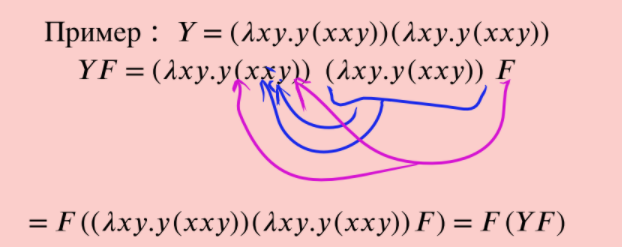
\includegraphics{images/3 (определения)_m32.PNG}
\end{center}

    \newpage
    \section{Простые утверждения}

\subsection{Композиция вычислимых функций вычислима.}
Пусть машина $M_f$ вычисляет функцию $f$, а машина $M_g$ — функцию $g$. Тогда функцию $f(g(x))$ можно вычислить машиной $M_g$, которая вместо своего конечного состояния переходит в начальное состояние машины $M_f$ (при этом для самой машины $M_f$ нужны новые состояния, не пересекающиеся с состояниями $M_g$).

\subsection{Существование невычислимых функций, неразрешимых и неперечислимых множеств (из соображений мощности).}
\textbf{Невычислимая}\\
Функции, о которых идет речь, представляют собой функции, заданные и принимающие значения в множестве слов в алфавите $A$. Ясно, что множество слов в алфавите $A$ счетно. Следовательно, рассматривается множество всех функций, заданных на счетном множестве и принимающих значения в счетном же множестве. Как известно, это множество имеет мощность континуума. С другой стороны, поскольку множество всевозможных машин Тьюринга счетно, то множество функций, вычислимых по Тьюрингу, также счетно. Континуальная мощность строго больше счетной. Следовательно, существуют функции, не вычислимые по Тьюрингу.

\textbf{Неразрешимое и неперечислимое множество}\\
Алгоритмов (и поэтому разрешимых/перечислимых подмножеств натурального ряда) счётное число, а всех подмножеств натурального ряда несчётное число. Значит, из соображения мощности найдутся неразрешимые и неперечислимые множества.

\subsection{Разрешимость любого конечного множества.}
Алгоритм разрешения любого конечного множества $S$ содержит таблицу элементов множества $S$, вход сравнивается по очереди со всеми элементами таблицы. В случае совпадения выдаем $1$, иначе $0$.

\subsection{Перечислимость любого разрешимого множества.}
По определению разрешимого множества, существует такая машина, что если $x \in A$, то существует вычисление, начинающееся в $q_1x$ и заканчивающееся в $q_a$. Это значит, что для этой машины все $x \in A$ встречаются в потоке вывода. Значит, множество A перечислимо.

\subsection{Замкнутость классов разрешимых и перечислимых множеств относительно пересечения, объединения, декартова произведения и конкатенации, класса разрешимых относительно дополнения и разности.}
\textbf{Пересечение и объединение перечислимых множеств -- перечислимое множество}
\\
Если $X$ и $Y$ перечисляются алгоритмами $A$ и $B$, то их объединение перечисляется алгоритмом, который параллельно выполняет по шагам $A$ и $B$ и печатает всё, что печатают $A$ и $B$. С пересечением немного сложнее -- результаты работы $A$ и $B$ надо накапливать и сверять друг с другом; что появится общего -- печатать.

\textbf{Пересечение, объединение, дополнение разрешимых множеств -- разрешимое множество}\\
Пересечение, объединение, дополнение -- это просто композиция соответствующей характеристической функции и булевой функции.
\begin{itemize}
    \item Для дополнения достаточно рассмотреть тот же алгоритм, что я для разрешения множества $A$. Вместо единицы печатать $0$, вместо $0$ -- единицу.
    \item $\chi_{A \cup B}(x) = \chi_A \vee \chi_B$ -- вычислима.
    \item $\chi_{A \cap B}(x) = \chi_A \wedge \chi_B$ -- вычислима.
\end{itemize}

\subsection{Существование вычислимой в обе стороны биекции между $\mathbb{N}^2$ и $\mathbb{N}$.}
$(x,y) \mapsto (2x + 1)2^y$

Это биекция -- очевидно, так как любое число представимо таким образом, причем разным числам соответствуют разные представления, и для любого числа вида $(2x + 1)2^y$ найдется число из $\N$. Опишем алгоритм вычисления:
\begin{itemize}
    \item[$\Rightarrow$] Очевидно, такая функция вычислима, как функция от двух аргументов.
    \item[$\Leftarrow$] Делим число на $2$, пока оно четно. Получаем отсюда $y$. Потом вычитаем один, делим на $2$, получаем $x$. 
\end{itemize}
Таким образом, построенная биекция вычислима в обе стороны, а значит, подходит под условие.

\subsection{Подмножество разрешимого (перечислимого) множества не обязательно разрешимо (перечислимо), и наоборот.}
\textbf{Подмножество разрешимого/перечислимого множества может быть неразрешимо/неперечислимо.}
Любое множество, в том числе неразрешимое/неперечислимое, является подмножеством $\mathbb{N}$, которое разрешимо/перечислимо.

\textbf{Подмножество неразрешимого/неперечислимого множества может быть разрешимо/перечислимо.}
Достаточно в любом множестве выбрать конечное подмножество, тогда оно разрешимо/перечислимо.

\subsection{Свойства m-сводимости: транзитивность, сводимость дополнений, разрешимость множества, m-сводимого к разрешимому, перечислимость множества, m-сводимого к перечислимому, сводимость разрешимого множества к любому нетривиальному.}
\begin{center}
    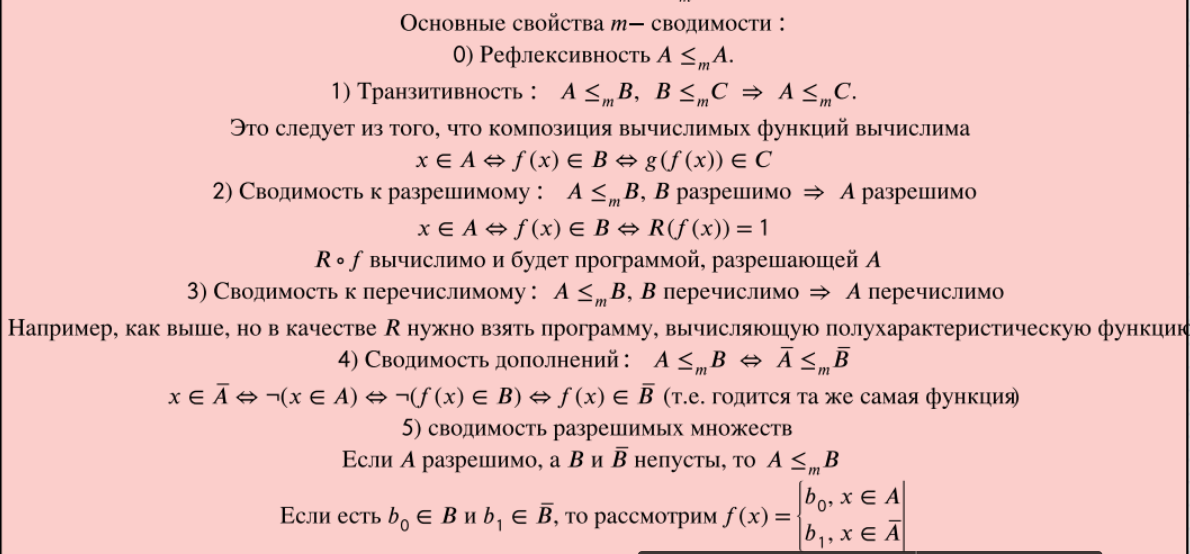
\includegraphics[width = 17cm, height = 8cm]{images/3 (определения)_m34.PNG}
\end{center}

\subsection{Вложенность классов в арифметической иерархии.}
$\Sigma_k \subset \Sigma_{k+1}, \Sigma_k \subset \Pi_{k+1}, \Pi_k \subset \Sigma_{k+1}, \Pi_k \subset \Pi_{k+1}.$\\
$ \blacktriangle$ Добавляем нужный квантор по фиктивной переменной. Например, $\exists y (x,y) \in R \lra \exists y \forall z (x,y,z)\in R \times \mathbb{N} \lra \forall t \exists y (x,y,t) \in R\times \mathbb{N}$ (из $\Sigma_1$ в $\Pi_2, \Sigma_2$). $\ \blacksquare$

\subsection{Замкнутость классов арифметической иерархии относительно объединения и пересечения.}
Пусть $A,B \in \Sigma_k$. Тогда:
\begin{center}
    $x \in A \Leftrightarrow \exists y_1\ \forall y_2 \ldots \exists y_k (x,y_1,\ldots,y_k) \in R$ \\
    $x \in B \Leftrightarrow \exists z_1\ \forall z_2 \ldots \exists z_k (x,z_1,\ldots,z_k) \in Q$
    \\
    $x \in A \cap B \ \lra (\exists y_1\ \forall y_2 \ldots \exists y_k (x,y_1,\ldots,y_k) \in R) \ \vee \ (\exists z_1\ \forall z_2 \ldots \exists z_k (x,z_1,\ldots,z_k) \in Q)  \lra \ \exists(y_1,z_1) \forall (y_2,z_2) \ldots \exists(y_k,z_k)((x,y_1,\ldots,y_k) \in R \wedge (x,z_1,\ldots,z_k) \in Q)$,
\end{center}
что является разрешимым свойством следующего кортежа: ($(x,(y_1,z_1),\ldots,(y_k,z_k)$).\\ Значит, $A \cap B \in \Sigma_k$. Для объединения аналогично.

\subsection{Дополнение языка из $\Sigma_{k}$ лежит в $\Pi_{k}$, и наоборот.}

Докажем, что дополнение языка из $\Sigma_{k}$ лежит в $\Pi_{k}$, обратное утверждение доказывается аналогично. По определению, множество $A $ принадлежит классу $\Sigma_n$, если существует такое разрешимое множество $R \in \mathbb{N}^{k+1}$, что
$$x \in A \lra \exists y_1 \ \forall y_2 \ \exists y_3 \ldots. \mathcal{Q} y_n [(x, y_1,\ldots,y_k) \in R].$$
Рассмотрим дополнение $\overline{A}$ к множеству $A$. Возьмем отрицание условия из определения:
$$ x \in \overline{A} \lra \forall y_1 \ \exists y_2 \ \forall y_3 \ldots. \overline{\mathcal{Q}} y_n [(x, y_1,\ldots,y_k) \in \overline{R}].$$
Так как дополнение разрешимого множества разрешимо, то $\overline{R}$ разрешимо, значит мы получили, что $\overline{A}$ принадлежит классу $\Pi_{k}$ по определению, что и требовалось.

\subsection{Пример $\lambda$-терма, к которому можно применить $\beta$-редукцию только после $\alpha$-конверсии.}
$(\lambda xy.x)y \underset{\alpha}{\Rightarrow}(\lambda xt.x)y \underset{\beta}{\Rightarrow}\lambda t.y$

\subsection{Пример $\lambda$-терма, не имеющего нормальной формы} $(\lambda x.xx)(\lambda x.xx)$

\subsection{Построение комбинаторов сложения и умножения для нумералов Чёрча (с доказательством корректности).} 
Add -- сложение.\\
$Add \ \overline{mn}$= $(\lambda mn fx. mf(nfx))\overline{m}\overline{n} = (\lambda n fx.\overline{m}f(nfx))\overline{n} = (\lambda n fx.(\lambda gy.\underbrace{g(g\ldots(g}_{m}y)\ldots))f(nfx))\overline{n} = (\lambda n fx.(\lambda y.\underbrace{f(f\ldots(f}_{m}y)\ldots))(nfx))\overline{n} = \lambda fx.(\lambda y.\underbrace{f(f\ldots(f}_{m}y)\ldots))(\overline{n}fx) = \\ \lambda fx.(\lambda y.\underbrace{f(f\ldots(f}_{m}y)\ldots))(\lambda gt.\underbrace{g(g\ldots(g}_{n}t)\ldots))fx) =  \lambda fx.(\lambda y.\underbrace{f(f\ldots(f}_{m}y)\ldots))(\underbrace{f(f\ldots(f}_{n}x)\ldots))) = \\ \lambda fx.(\underbrace{f(f\ldots(f}_{m + n}x)\ldots)) = \overline{m} +\overline{n}$. \\

Mult -- умножение:\\
$Mult \ \overline{mn} = (\lambda mn fx. m(nf)x)\overline{mn} =  (\lambda n fx. \overline{m}(nf)x)\overline{n} = (\lambda n fx. (\lambda gy.\underbrace{g(g\ldots(g}_{m}y)\ldots))(nf)x)\overline{n} \\ = \lambda fx. (\lambda gy.\underbrace{g(g\ldots(g}_{m}y)\ldots))(\overline{n}f)x = \lambda fx. (\lambda y.\underbrace{\overline{n}f(\overline{n}f\ldots(\overline{n}f}_{m}y)\ldots))x = \\ \lambda fx. (\lambda y.\underbrace{\overline{n}f(\overline{n}f\ldots\overline{n}f(\lambda g t_1. \underbrace{g(g\ldots(g}_{n}t_1)\ldots))f}_{m}y)\ldots))x \\ = \lambda fx. (\lambda y.\underbrace{\overline{n}f(\overline{n}f\ldots\overline{n}f}_{m-1}(\underbrace{f(f\ldots(f}_{n}y)\ldots)))\ldots))x  = \lambda fx. (\lambda y.\underbrace{\overline{n}f(\overline{n}f\ldots\overline{n}f}_{m-2}(\underbrace{f(f\ldots(f}_{n + n}y)\ldots)))\ldots))x = \ldots = \\ \lambda fx. (\lambda y.(\underbrace{f(f\ldots(f}_{n*m}y)\ldots)))\ldots))x = \lambda fx.\underbrace{f(f\ldots(f}_{n*m}x)..) = \overline{m}*\overline{n} $.
    \newpage
    \section{№3 Изоморфизм группы}

\begin{reminder}
  наименьшее k --- порядок группы, если $g ^ k = e$.
\end{reminder}

\begin{note}
  $(Z_n, +) \quad \ord a = \frac{n}{\gcdru(a, n)}$
  \[S_n \ord \Pi = \gcdru(\text{\#len}).\] Где \#len --- длинна циклов.
\end{note}

\subsection{Порядки перестановки}

\begin{reminder}
  $\Pi: (a_0, a_1, \dots, a_{l - 1})$. Если $\Pi ^ {s} = \id \Ra \Pi ^{s} (a_0) = a_0 \Ra l \mid s$
  \[\ord \Pi = l.\]
\end{reminder}

\begin{example}
  $\pi = \underbrace{(\dots)}_{l_1}\underbrace{(\dots)}_{l_2}\underbrace{(\dots)}_{l_3} \dots \underbrace{(\dots)}_{l_s}$. Тогда имеем $\ord \pi = \gcdru(l_1, \dots, l_s).$
\end{example}

\begin{example}
  $\mid G \mid = n, \ d = 80, \ \mid S_{12} \mid = 12!$
  \[\gcdru(l_1, \dots, l_s) = 80, \]
  \[l_1 + \dots + l_s = 12.\]
  То есть невозможно.
\end{example}

\subsection{Основная теорема арифметики}
\begin{theorem}[Основная теорема арифметики]
  Для любого n > 1 --- \ul{однозачно} представялется произведением простых множителей (с точностью до пересестановки множителей).
\end{theorem}

\begin{example}
  $80 = 2 ^ 4 \cdot 5 = 2 ^ 2 \cdot 5 \cdot 2 ^ 2$.
\end{example}

\begin{proof}
  По индукции. $n = 2$ --- база. Пусть < n --- существует.
  \begin{enumerate}
    \item[(1)] n --- простое,
    \item[(2)] $n = ab, \ 1 < a, b < n$.
  \end{enumerate}
  Пусть $x \not \equiv 0 \mod p \Ra x^{-1} \cdot x \equiv 1 \mod p \Ra y \equiv 0 \mod (p)$.
\end{proof}

\begin{lemma}
  p --- простое, то есть $xy \equiv 0 \mod (p) \Ra$
  \[x \equiv 0 \mod (p) \vee y \equiv 0 \mod (p).\]
\end{lemma}

\begin{proof}
  $\underbrace{p_1 \dots p_k}_{\text{Делится на } p_1} = q_1 \dots q_s$, где $p_i, q_j$ --- простое. Тогда утверждается, что $p_i \not = q_i$ --- в силу закона сокращения.
  \[\Ra p_1 \mid q_k \Ra p_1 = q_k.\] В силу того, что левая часть делится на $p_1$.
\end{proof}

\begin{proposition}
  $n = p_1^{a_1} \dots p_t^{a_t} \dots, \quad p_1 < p_2 < p_3 < \dots < p_t < \dots$
  \[p_k \nmid n \Ra a_k = 0.\]
\end{proposition}

\begin{example}
  \[x = p_1^{a_1} \dots p_t^{a_t} \dots ,\]
  \[y = p_1^{b_1} \dots p_t^{b_t} \dots ,\]
  \[x \mid y \Lra a_i \leq b_i,\]
  \[\gcdru(x, y) = p_1^{\min (a_1, b_1)} \cdot \ldots \cdot p_t^{\min (a_t, b_t) },\]
  \[\lcm(x, y) = p_1^{\max (a_1, b_1)} \cdot \ldots \cdot p_t^{\max (a_t, b_t) }.\]
\end{example}

\subsection{Класс групп}
\begin{definition}
  Группа G --- циклическая, если:
  \[G = \langle g \rangle.\]
  Обозначение: $C_n$ --- циклическая.
\end{definition}

\begin{corollary}
  Любая циклическая группа --- абелева. То есть, для любого элемента выполнено: $g^{i + j} = g^i \cdot g^j$.
\end{corollary}

\begin{example}
  $| (Z_{\delta}^{\text{*}}, \cdot) | = 4, \quad 1^2 \equiv 3^2 \equiv 5^2 \equiv 7^2 \equiv 1 \mod \delta$.
\end{example}

\begin{theorem}
  Если, $G = \{ g^i, i \in \ZZ \} = \langle g \rangle$, то изоморфны и $(\ZZ, +)$ и $(Z_n, +)$.
\end{theorem}

\begin{example}
  $|G| = \infty$ --- все степени различны.
  \[g^i = g ^ j \Lra g^{j - i} = e,\]
  \[k \raone g^k,\]
  \[(\ZZ, +) \ra G,\]
  \[g^{n + qn} = g^i \cdot g^{qn} = g^i \cdot (g^n)^q.\]
\end{example}

\begin{theorem}
  Подгруппа циклической группы --- циклическая.
\end{theorem}

\begin{example}
  Пусть $G < (\ZZ, +)$, тогда 
  \[\quad d = \min (x: x > 0 \quad x \in G), \]
  \[g \in G \quad g = qd + r, \ 0 \leq d, \]
  \[t = g - qd \in G \Ra r = 0.\]
  Если $G < (Z_n, +)$, тогда
  \[d  = \min (x: 0 < x < n \quad [x] \in G),\]
  \[d \mid n \quad n = qd + r \Ra r \in G \Ra r = 0.\]
\end{example}

\subsection{Изоморфизм групп}
\begin{example}[1]
  $(Z_6, +)$. Нейтальный --- $0$. Кратные элементы --- $ka$.
\end{example}

\begin{example}[2]
  $g = \langle(12)(345)\rangle, \quad \ord g = 6$
\end{example}

\begin{definition}
  Изоморфизм групп, это отображение, такое что:
  \[\phi : G_1 \ra G_2\]
  \begin{enumerate}
    \item[(1)] $\phi$ --- биекция,
    \item[(2)] $\phi(xy) = \phi(x) \ \phi(y)$. Для любых $x, y \in G$.
  \end{enumerate}
  Обозначение: $G_1 \cong G_2$.
\end{definition}

\begin{note}
  Тогда имеем, что примеры (1) и (2) --- изоморфны.  
\end{note}

\subsection{Прямое произведение групп}
\begin{definition}
  Пусть G, H --- группы. Тогда, $G \times H = \{(g, h): g \in G, h \in H\}$. Тогда имеем несколько свойств: 
  
  \begin{enumerate}
    \item $(g_1, h_1) \cdot (g_2, h_2) = (g_1 \cdot g_2, h_1 \cdot h_2)$,
    \item $\ord (g, h) = \lcm(\ord g, \ord h)$,
    \item $(g, h)^k = (g^k, h^k) = (e, e)$.
  \end{enumerate}
\end{definition}

\begin{proposition}
  $\gcdru(p, q ) = 1$, тогда имеем: $C_p \times C_q \cong C_{pq}$.
\end{proposition}

\begin{proof}
  $\ord(1, 1) = \gcdru(p, q) = \frac{pq}{1} = pq = |C_p \times C_q|$.
\end{proof}

\begin{corollary}
  $C_p \times C_q \text{--- циклическая} \cong C_{pq}$.
\end{corollary}

\subsection{Мультипликативность функции Эйлера}

\begin{proposition}
  % $\gcdru(p, q) = 1 \Ra \underbrace{\phi(pq)}_{\text{Число порождающих в } C_{pq}} = \underbrace{\phi(p) \phi (q)}_{\text{Число порождающих в } C_p \times C_q}$
  Если $\gcdru(p, q) = 1$, то выполено равенство:
  \[\phi(pq) = \phi(p) \phi (q).\]

  % $\phi(n) = |(Z_n^{\text{*}}, \cdot)|$
\end{proposition}

\begin{proof}
  Равенство верное, в силу того, что левая часть --- число порождающих в $C_{pq}$, а справа --- число порождающих в $C_p \times C_q$.
\end{proof}

\begin{proposition}
  Количество пораждающих в $C_n$ равно $\phi(n)$.
\end{proposition}

\begin{proof}
  \[(x, y) \in C_p \times C_q, \]
  \[\ord (x, y) = \gcdru(\ord x, \ord y) = pq \Ra \ord x = p, \quad \ord y = q.\]    
\end{proof}

\begin{example}
  Пусть $n = p_1^{q_1} \dots p_t^{a_t}, \quad a_i > 0$, тогда

  \[\phi (p^n) = p^n - p^{n - 1}.\]В силу того, что $x \not \equiv 0 \mod (p^n) \Lra x \equiv 0 \mod (p)$.

  \[\phi(n) = (p_t^{a_t} - p_t^{a_t - 1}) = n (1 - \frac{1}{p_1}) (1 - \frac{1}{p_2}) \dots (1 - \frac{1}{p_t}).\]
\end{example}


    
\end{document}